%\documentclass{sig-alternate-10pt}

\documentclass[10pt, conference, letterpaper]{IEEEtran}


%\usepackage{txfonts}
\usepackage{amsmath}
%\usepackage{mathbold}
\usepackage{cases}

% correct bad hyphenation here
\hyphenation{op-tical net-works semi-conduc-tor}


\usepackage{cite}
\usepackage{times}
\usepackage{graphicx}
\usepackage{graphics}
\usepackage{subfigure}
\usepackage{epsfig}
\usepackage{latexsym}
\usepackage{amsfonts}
\usepackage{amssymb}
\usepackage{paralist}
\usepackage{xspace}
\usepackage{mathrsfs}
\usepackage{amssymb}
\usepackage{slashbox}
%\usepackage{setspace}
\usepackage{color}
%\usepackage[linesnumbered,ruled,vlined]{algorithm2e}
 %\usepackage{algorithmicx}
 %\usepackage{algpseudocode}
\usepackage{algorithm} %ctan.org\pkg\algorithms
\usepackage{algorithmicx}
\usepackage{algpseudocode}
\usepackage{amsmath}
\usepackage{url,epsfig,array}
\usepackage{setspace}
%\usepackage{fontspec}

\renewcommand{\ttdefault}{cmtt}

%\usepackage{listings}

%\lstset{language=C++}
%\lstset{breaklines}
%\lstset{extendedchars=false}


\allowdisplaybreaks %%% this make pages look tight.
%%%%%%%%%%%%%%%%%%%%%%%%%%%%%%%%
\def\ie{\textit{i.e.}\xspace}
\def\etal{\textit{et al.}\xspace}
\def\etc{\textit{etc.}\xspace}
\def\whp{\textit{w.h.p.}\xspace}
\def\eg{\textit{e.g.}\xspace}
\def\iid{\textit{i.i.d.}\xspace}
\def\st{\xspace\textbf{s.t.}\xspace}

\def\accl{\textbf{a}}
\def\oursystem{\xspace{PerLoc}\xspace}
\newcommand{\CUTXY}[1]{{}}

\newcommand{\mynote}[1]{{$\langle${\textbf{\textcolor{blue}{#1}}}$\rangle$}}
\newcommand{\linote}[1]{{$\langle${\textbf{\textcolor{red}{#1}}}$\rangle$}}

\newcommand{\weight}[2]{{\omega(#1,#2)}}
\newcommand{\length}[1] {{\Vert #1 \Vert}}
\newcommand{\prob}[1]{{\textbf{Pr}\left(#1\right)}}
\newcommand{\link}{{\textbf {L}}}

\renewcommand{\paragraph}[1]{\smallskip \noindent {\textbf{#1}}}
\renewcommand{\algorithmicrequire}{\textbf{Input:}}
\renewcommand{\algorithmicensure}{\textbf{Output:}}
\newtheorem{theorem}{Theorem}
\newtheorem{axiom}[theorem]{Axiom}
\newtheorem{corollary}[theorem]{Corollary}
\newtheorem{definition}{Definition}
\newtheorem{lemma}[theorem]{Lemma}
\newtheorem{remark}[theorem]{Remark}
\newtheorem{proposition}[theorem]{Proposition}
% defines environments: theorem, lemma, proposition, corollary



% the proof environment
%\newenvironment{proof}[1][Proof]{\begin{trivlist}
%\item[\hskip \labelsep {\bfseries #1}]}{\end{trivlist}}


\begin{document}
\title{PerLoc: Enabling Infrastructure-Free Indoor Localization with Perspective Projection }
%\author{IEEE Infocom 2015. Paper ID}


%\author{Puchun Feng,Lan Zhang, Kebin Liu, Yunhao Liu}
\author{\IEEEauthorblockN{Puchun Feng, Lan Zhang, Kebin Liu, Yunhao Liu }
\IEEEauthorblockA{School of Software and TNLIST, Tsinghua University \\
Email: fengpc12@mails.tsinghua.edu.cn, \{zhanglan, kebin, yunhao\}@greenorbs.com}
}
%\thanks{This work is supported by .}\\
%       \affaddr{Tsinghua University, Beijing, China}\\
%       \email{zhanglang03@gmail.com}}
%\thanks{This research was partly funded by the National 863 Plan (Projects Numbers: 2009AA04Z153), P. R. China, and The State Key Development Program for Basic Research of China (Grant No.  2010CB328000).}


\maketitle


\begin{abstract}
With the rapid development of mobile applications, there is an urgent need for highly efficient indoor localization service.
Dedicated systems achieve good accuracy at the cost of deploying special hardware. Fingerprint-based methods avoid maintaining the expensive infrastructure but suffer from intensive labor for site-survey and poor robustness.
In this paper, we present \oursystem, an infrastructure-free localization system which leverages rich vision features in indoor environment with high efficiency and accuracy. \oursystem makes use of binocular ranging technique to calculate the depth of a feature point and then figures out its geographical coordinates to build up reference point database, for which we design a filtering scheme to keep the database efficient in storage and search delay. During the localization stage, users simply take a photo of surroundings and feature points are extracted automatically as input for search scheme. Then a fast two-stage search scheme is proposed to find the nearest neighbors of query feature points in reference point database. Based on the perspective projection model, we inversely calculate users' geographical location in realtime.
We implement the proposed localization system on commercial smartphones as well as laptops and conduct extensive experiments. \oursystem achieves $1.76m$ of average error in office environment, and $2.2m$ of average error in shopping mall.


\end{abstract}

\section{Introduction}
\label{sec:introduction}
Worldwide user base of smartphone hit 1 billion in 2012 and the current number of apps available in Apple's AppStore exceeds 700,000,
 meanwhile there is about the same number of live Android apps in the market.
Accurate localization service is a fundamental service for a significant portion of these applications. While the outdoor localization has been solved by GPS, localization in indoor environment remains an open question, leading to largely restricted adoption of many apps for indoor scenarios.
Although numerous research studies as well as industrial efforts have been devoted to this problem, heretofore there still lacks a feasible and widely applied approach for indoor localization.
%Nowadays, research on indoor localization service attracts more and more attention.
Existing work can be generally classified into two categories. One category includes many dedicated systems that require deploying infrastructure \cite{borriello2005walrus}\cite{hazas2005relative} in priori or leveraging specialized hardware \cite{prorok2011accommodation}\cite{priyantha2000cricket}.
These methods have achieved high accuracy but can hardly be applied on smartphones whose demands are stringent. Besides, they suffer from expensive infrastructure resulting in the difficulty of scaling to pervasive usage. The other category of solutions is infrastructure-free. Most of extant infrastructure-free approaches use fingerprints to index locations, where they are collected, and build fingerprint databases. On the localization stage, user's smartphone senses fingerprints which are then compared with ones stored in database. Then the location label of the best matched fingerprint is returned to the user. The most commonly applied fingerprints are WiFi signals from prevalent wireless access points.
These methods, however, still have some limitations for practical applications. First, they need exhausted survey of wireless fingerprints on all locations, which is very costly. To fulfill this task, crowdsourcing methods \cite{yang2012locating} are considered in recent works. Second, these schemes suffer a lot from the dynamics of signal distribution. For example, the displacement of an access point can significantly degrade their performance. Finally, although reasonable accuracy can be achieved, fingerprint-based approaches can have significant errors due to one of their fundamental limits, distinct locations with similar signatures. Some researchers propose to use image matching which determines the user's location by searching the most similar images in database and then returns the location where the matched image is surveyed. These methods incur large amounts of storage cost to maintain image database with very high delay for image searching. Furthermore, they can only provide room-level accuracy due to the sparse sampling.

To address these issues, we present \oursystem, a novel type of infrastructure-free indoor localization system, which explores the rich and stable vision features of the indoor environment and makes use of the geographical information of these vision features to inversely calculate user's location.
Site-survey of \oursystem is conducted only at a few locations by taking photos of indoor environment with two cameras and then we extract vision features from photos. We leverage the binocular ranging technique to calculate the depths of vision features, which are used to figure out vision features' geographical coordinates. We propose a two-stage, cluster-based search scheme to fast find the nearest neighbors of user's query feature points. On the localization stage, according to perspective projection model we avail of query features' nearest neighbors to inversely calculate user's geographical location in realtime and with high accuracy.
As an infrastructure-free indoor localization system, \oursystem avoids the limitations of existing fingerprinting schemes and exhibits the following advantages:
1) Lightweight and easy to operate site-survey. Different from fingerprinting, our method does not require an exhaustive site-survey, with only a few locations surveyed for generating reference points.
2) Robust. The vision features leveraged in this work are highly distinctive, invariant to scale, rotation, distortion, addition of noise, change in viewpoint, and change in illumination and thus avoid the impact of dynamic signal distribution.
3) Highly accurate and realtime. \oursystem achieves $1.76m$ of average error in office environment, and $2.2m$ of average error in shopping mall. In office environment \oursystem only takes no more than $1.5s$ for 90\% queries, $1s$ for 90\% in shopping mall and the average time is no more than $1.5s$ for both.

The major contributions of this work are summarized as follows:
\begin{itemize}
\item We present a new framework leveraging vision features to achieve highly efficient indoor localization. Based on the perspective projection model, we inversely calculate the geographical location of a user in realtime.
\item We enhance the performance of inverse localization by the optimization of the error estimate function, which appends a vote procedure to select the final result.
\item We propose an integrated system design including novel approach for vision based site-survey, fast search scheme for the query feature's nearest neighbor and inversely calculation of user's location.
\item We implement the proposed scheme on both smartphone and PC, and also conduct extensive experiments to verify the effectiveness of our approach.


\end{itemize}
The rest of the paper is organized as follows. Section 2 introduces the system architecture. Section 3 presents the consideration and design of site-survey approach. Section 4 describes the two-stage search scheme. Section 5 elaborates the algorithm of inverse localization and optimization about it. The performance is evaluated in Section 6 and related work is summarized in Section 7. Finally we concludes this paper in Section 8.

%
%
%\mynote{challenges of our approach}
%\mynote{the FM paper}
%
%Advantages:
%\begin{itemize}
%\item Vision features are highly distinctive�� invariant to scale, rotation, distortion, addition of noise, change in viewpoint, and change in illumination.
%\item Angle of view is consistency for same devices.
%\item Rich vision features provide high robustness and uniqueness.
%\item Infrastructure-free and good devices compatibility.
%\item Easy construction and deployment for any environment.
%\item High accuracy of both location and orientation.
%\item Low computation, communication and storage cost.
%\end{itemize}


\section{System Overview}
\label{sec:over}
In this section, we provide a brief overview of \oursystem architecture as shown in Figure~\ref{overview}. \oursystem firstly builds up reference point database which stores the geographical information of reference points together with vision descriptors extracted by the site survey component. When a user sends query feature points extracted by the querier component to the server, the search component finds the nearest neighbors of query features by two-stage search scheme. At last, the localization component inversely calculates the user's location and sends the result to the user.
\begin{figure}[!ht]
\centering
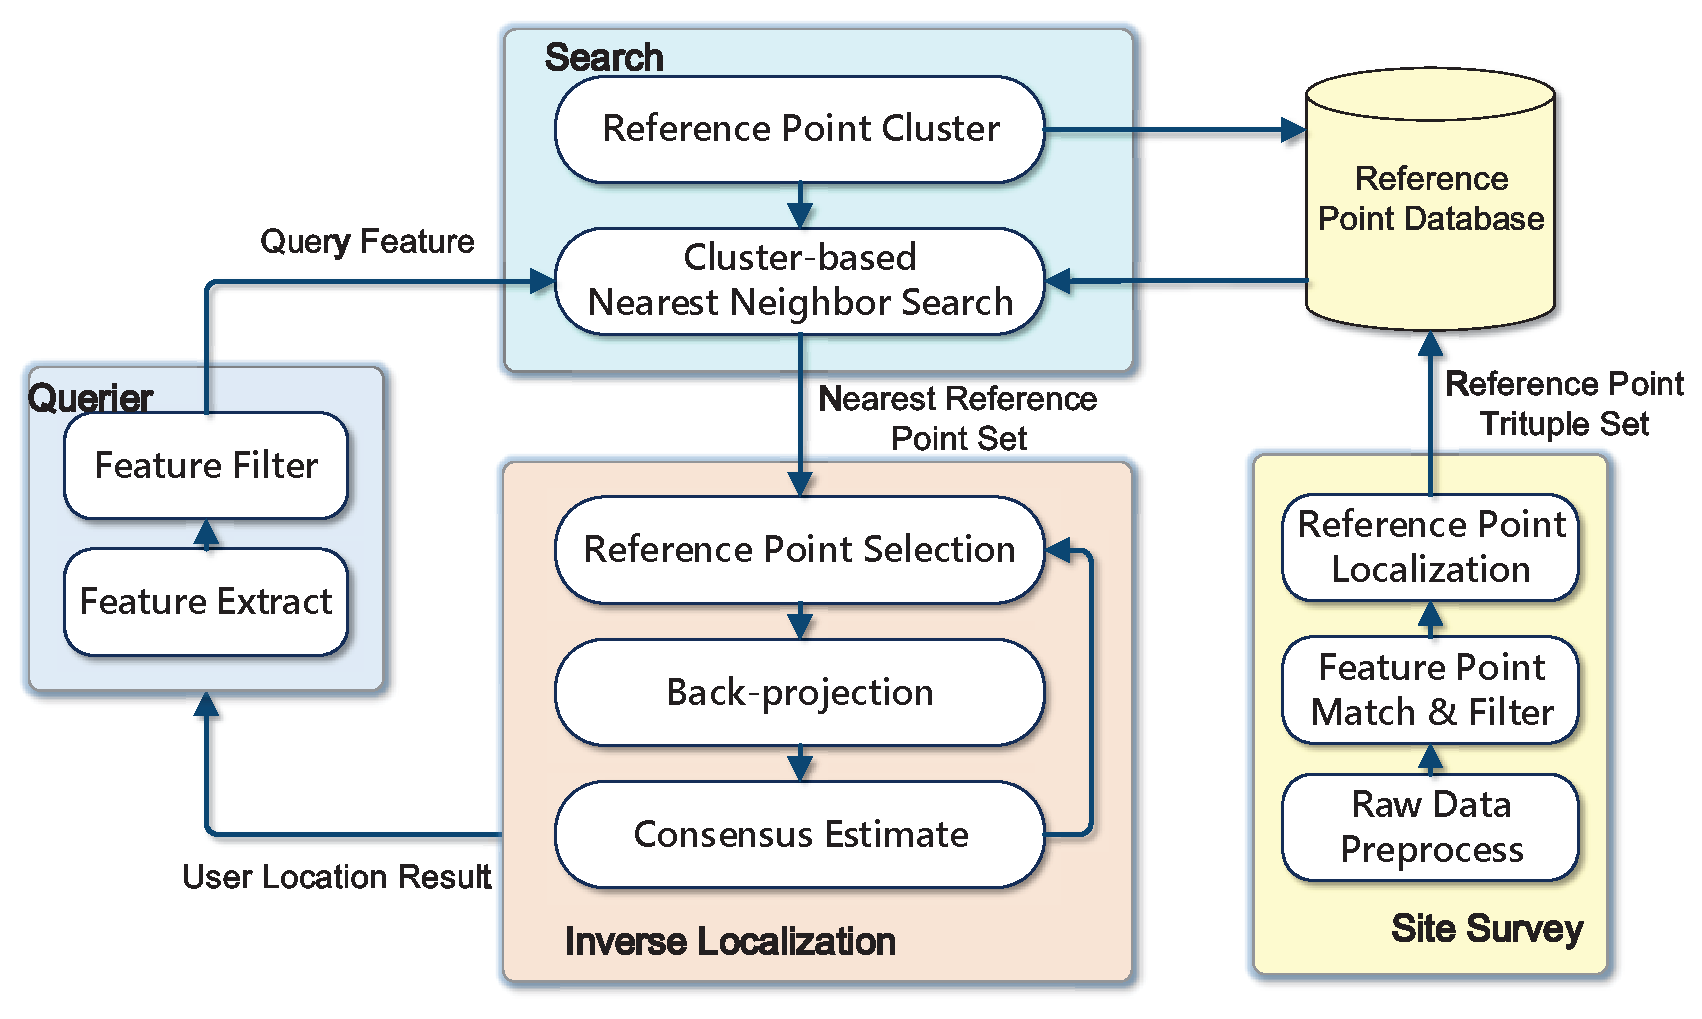
\includegraphics[width=1\linewidth, clip,keepaspectratio]{overview2.eps}
\caption{\oursystem system architecture.}\label{overview}
\end{figure}


\oursystem consists of four components:


\textbf{(1)Querier Component:}
This component runs on smartphone as an application for users. It extracts the feature points from the query photo taken by a user, and generates a descriptor for each feature point. But we don't need all feature points, for the reason of saving communication cost and filtering out the unstable feature points, \ie features not on building structures or features on people, which would decrease accuracy of localization.

\textbf{(2)Site Survey Component:}
Site survey component builds up the specific reference point database for a building. We calculate the geographical location of a reference point according to its depth which is figured out by binocular ranging. Binocular ranging makes use of the disparity of one feature point to calculate its depth. In order to obtain the disparity of feature points, we firstly take pair-photos(Figure~\ref{pair}) for the building on the predefined survey track. Then this component extracts feature points from pair-photos. It matches the feature point in the left photo to the most similar feature point in the right photo to calculate disparity of this feature. However, some matches are not similar enough or not reasonable, \eg one feature on the floor matches to one on the ceiling though their descriptors are similar. These bad matches should be thrown away because they may impact the calculation of geographical position of reference point. Then we indicate the geographical coordinates of feature point according to its depth and pixel coordinates. We combine the descriptor of a feature point with its geographical coordinates to form a reference point and store all of them into reference point database.

\textbf{(3)Search Component:}
\begin{figure}[t!]
\centering
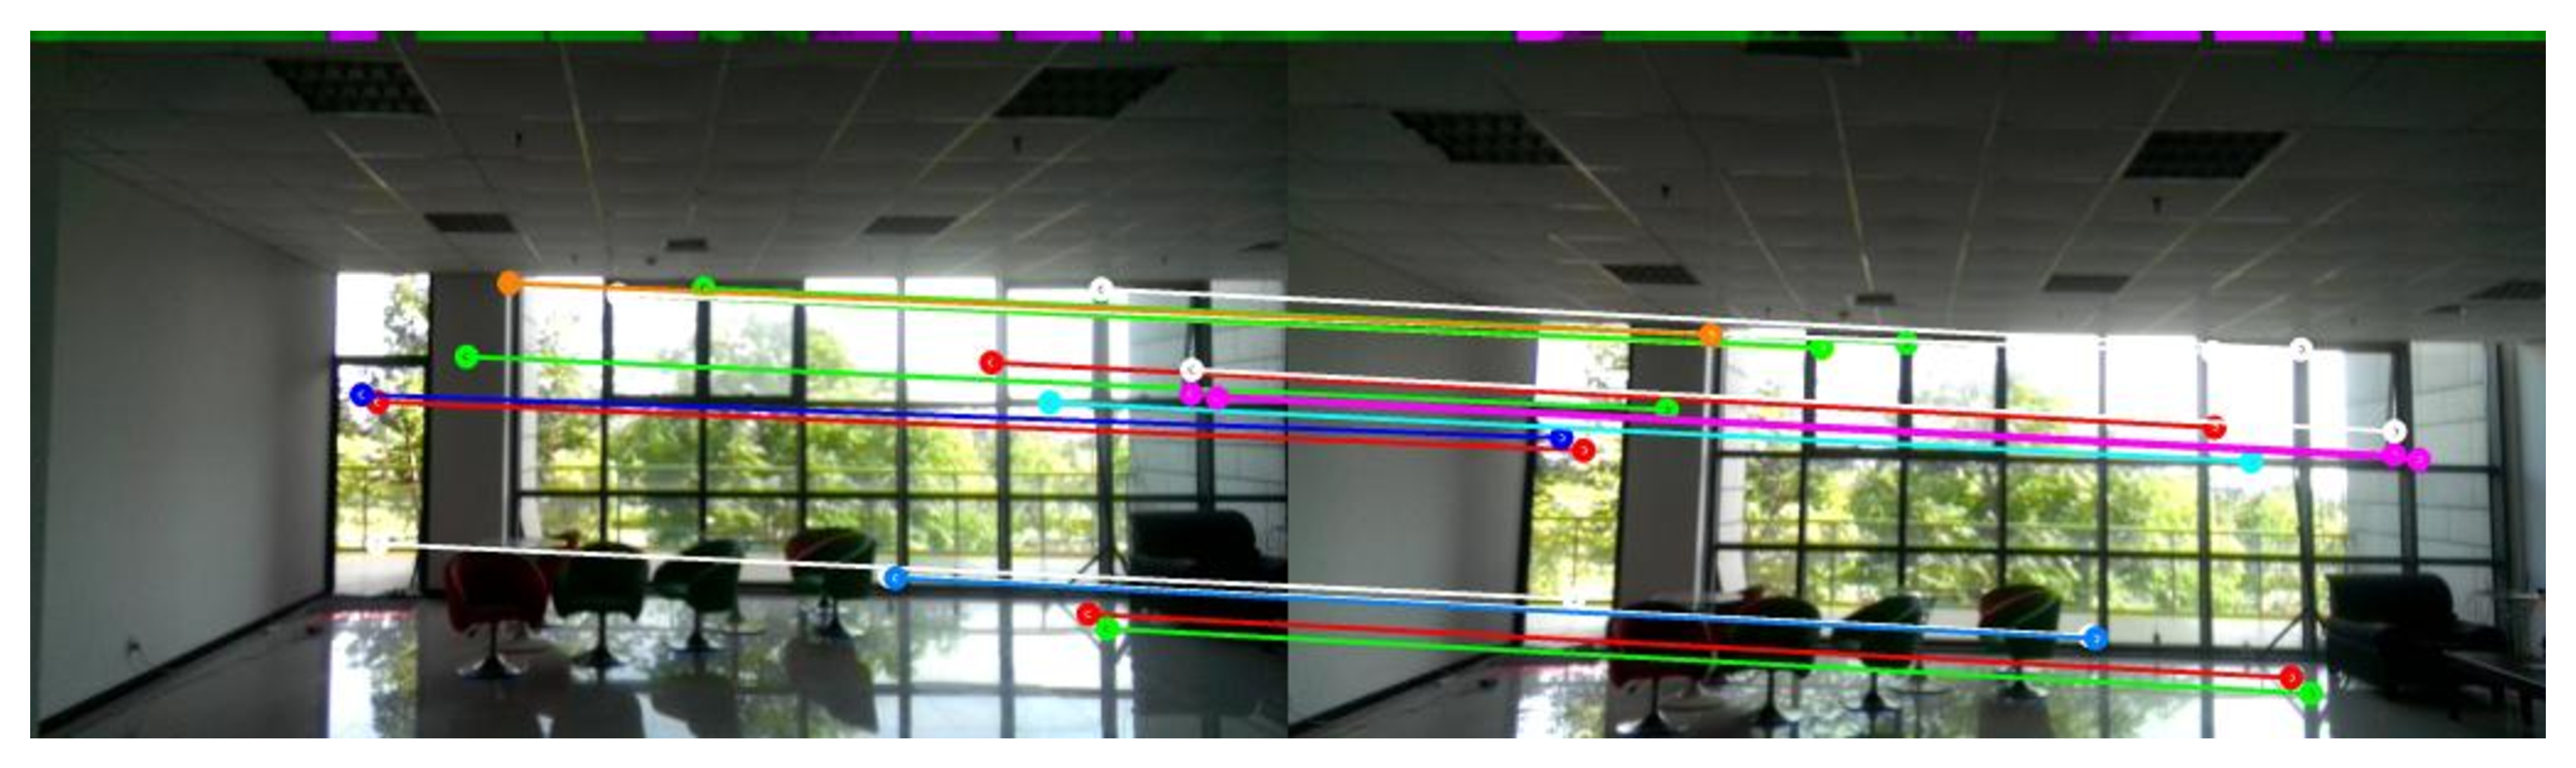
\includegraphics[width=1\linewidth, clip,keepaspectratio]{pair_photo.eps}
\caption{Pair-photo with feature point matches.}\label{pair}
\end{figure}
Given a localization request, the search module will find the nearest neighbor for each query feature descriptor using two-stage cluster-based search algorithm. The cluster-based search algorithm makes use of feature point clusters generated by reference point cluster component. One cluster consists of reference points whose feature descriptors are near to each other in Euclidean distance. In one cluster, we choose a reference point to represent all points in it and this representative can be treated as the centroid of cluster.

\textbf{(4)Inverse Localization Component:}
This component inversely calculates user's location as soon as the search component outputs the nearest neighbor set of query feature points. Firstly, we choose the trine of match from search component's outputs. Each trine contains three matches between query points and reference points. We sort these trines according to the similarity of matches measured by the distance between two feature points. The trine whose matches have high similarity will get high priority. We calculate the geographical location of user by solving the location determination problem(LDP). As we figure out a location, we estimate the error of location by calculating the consensus of it in its nearest neighbor set. The location with low consensus is possible to be inaccurate, so we discard it and start another round of inverse calculation. This process stops until the number of rounds exceeds the threshold. At last, this component returns the most accurate result of user's location.


\section{Site Survey Approach}
\label{sec:site}

The site-survey stage extracts and selects a set of reference points in the indoor environment then builds up a reference point database. Instead of collecting wireless fingerprints at all coordinates, in \oursystem we just extract feature points at only a few locations for the reason that at one shooting point we are able to collect many feature points as long as no obstacle lies between us and building structure. Each reference point stored in the database is denoted as a trituple $R = (v, c, a)$ where $v$ is a vector of vision features which we refer to as the \emph{feature descriptor} in this work, $c$ represents the geographical coordinates of the reference point and $a$ denotes the visible orientation of this reference point.
% Note that the visible orientation of a reference point is affected by both the obstacles (\eg we cannot see reference points behind a wall) and the angle of viewpoint.
In this work, we leverage the state-of-the-art feature detector SURF\cite{bay2006surf}, a performant scale- and rotation-invariant interest point detector and descriptor, which is inspired by the SIFT descriptor\cite{lowe2004distinctive}, and is faster than SIFT. With this typical setting, a SURF feature descriptor can be represented as a vector with 64 dimensions.
%SIFT achieves high performance in matching to large databases. As reported in \cite{lowe2004distinctive}, there are nearly 80\% of correct matches in a database with up to 100000 key points under the condition that images have random scale and rotation changes, an affine transform of 30 degrees, and noise of 2\% added in priori.
%As the users may turn on the localization component at anywhere inside the building, the surveyed reference points should be evenly distributed all-round the indoor environment. Note that as we conduct site-survey floor by floor and users usually take picture at similar altitudes on each floor, we consider the coverage problem only on horizontal direction.
\subsection{Observations of Site Survey}

We are aiming to collect reference points associated with the building structure for the reason that these features are relatively stable.
A straight-forward solution is to take pictures at consecutive locations, as shown in Figure~\ref{fig_site-survey}(a). Let $\alpha$ denote the view angle of the camera \ie the photo can cover reference points in a range of $\alpha$ degree.
This method ensures that all reference points be recorded from one direction.
However, there is another factor which should be considered, the visible orientation of the reference points which is denoted as $\beta$. Note that the SURF features retain high matching accuracy (80\%) out to a 30 degree change in viewpoint. In other words, if the users look at the same reference point from a direction that differs from that in site-survey stage for more than 15 degree, the reference point could be unrecognizable. Therefore, in this work, we set $beta$ to 30 degree.
As shown in Figure~\ref{fig_site-survey}(a), while standing in the shadow region the user will have difficulties in identifying reference points in front.
%To address this issue, we present a simple strategy to improve the visible orientation of reference points by adding more sampling locations.

There is no need to guarantee that all reference points can be identified from all directions, thus our design goal is to approximately ensure a proper view angle in front of each reference point, which means the reference point can be recognized from the direction orthogonal to its background building structure or even tolerates small skews in view angle. As $\beta$ is usually smaller than $\alpha$, we first consider $\alpha$ as wide as $\beta$ and set the distance between two shooting points to $D\cdot \tan(\frac{\beta}{2})$ as shown in Figure~\ref{fig_site-survey}(b). $D$ denotes the distance from the shooting point to the building structures. All reference points are covered by at least two pictures taken from adjacent points. The orange range of background is sampled at both $C_1$ and $C_2$ and the visible orientation of each reference point is the superposition of the visible orientations in two samples. By geometric analysis, all reference points in the overlapping range can be recognized from the direction orthogonal to the background with an angle skew less than $\frac{\beta}{2}$ to both clockwise and anticlockwise.
In practical usage, since $\alpha$ is usually larger than $\beta$ and we can take multiple pictures in different directions in one location, we have sufficient redundancies in the quantity of reference points to ensure the accuracy of query.
\begin{figure*}[!htpb]
\centering
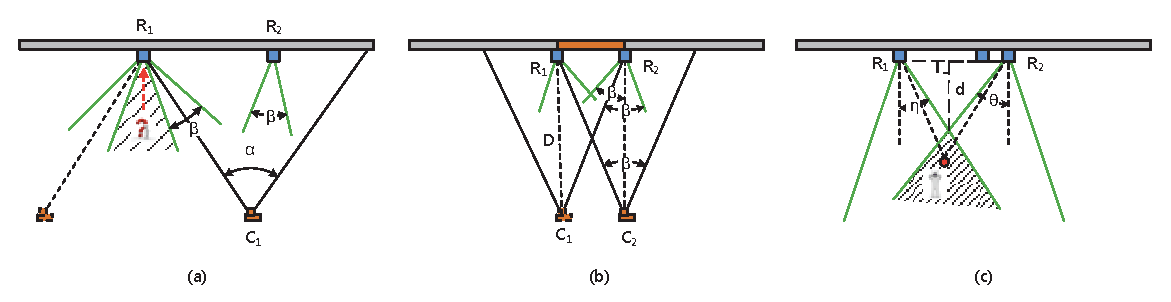
\includegraphics[width=1\linewidth,height=1.3in]{site-survey2.eps}
\caption{The observations of site-survey.}\label{fig_site-survey}
\end{figure*}
\subsection{Reference Points Geographical Coordinates Calculation}
Based on previous observations, we make a survey track according to the building structure. We annotate every shooting point in the track with its coordinates in the local coordinate system of the building. We take a pair-photo, including a left and a right photo,  at every shooting point. We use two cameras to take pair-photo, the left camera is $d_{cam}mm$ apart from the right camera.
\subsubsection{Depth Calculation}
Firstly, we will calculate the depth of feature point extracted from pair-photo using binocular ranging technique.
\begin{figure}[!hb]
\centering
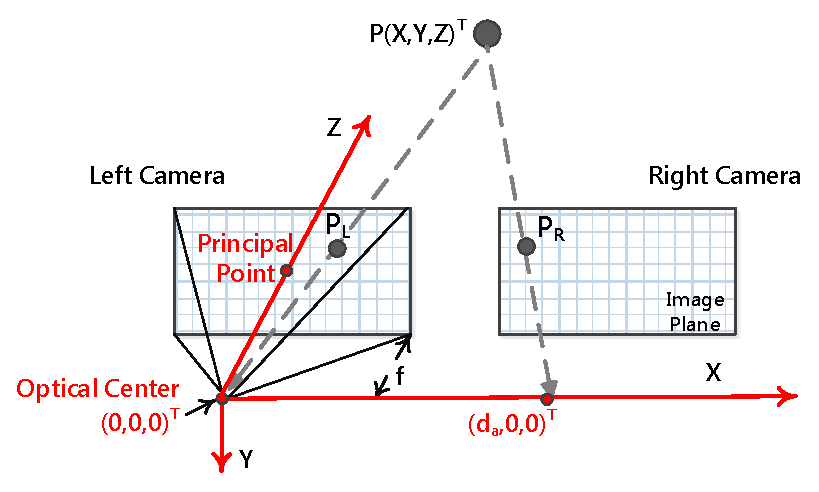
\includegraphics[ height=1.3in]{twoview2.eps}
\caption{Model of reference point's depth calculation.}\label{fig_twoview}
\end{figure}
Figure~\ref{fig_twoview} shows the geometry model of calculation for reference point's depth.
Optical center is the center of the perspective projection, the optical axis is perpendicular to the image plane piercing through the principal point on the plane.
Without loss of generality, the coordinate system is selected such that
 its origin is located at the optical center of the left camera
 and the Z-axis is collinear to the optical axis, as shown in Figure~\ref{fig_twoview}.
$P$ $(X,Y,Z)^T$ is a geographical coordinate of one feature point
 and the two corresponding projected pixels on image planes are $P_L$$(x_L,y_L)$ and $P_R$$(x_R,y_R)$, where $x_L$, $x_R$, $y_L$, $y_R$ denote pixel coordinates.
Let the principal point of left camera be $(o_x,o_y)^T$.
The projection of $P$ on the image plane of the left camera is
\begin{equation}
x_L = \frac{X\cdot f}{Z}+o_x, y_L = \frac{Y\cdot f}{Z}+o_y.
\end{equation}
Expressed in matrix:
\begin{equation}
\lambda_L \begin{pmatrix}x_L \\ y_L \\ 1 \end{pmatrix} = \begin{pmatrix}f & 0 & o_x\\0 & f & o_y\\ 0 & 0 & 1 \end{pmatrix} \begin{pmatrix}X \\ Y \\ Z\end{pmatrix}.
\end{equation}
$\lambda_L$ is a scaling factor.
Let $K=\begin{pmatrix}f & 0 & o_x\\0 & f & o_y\\ 0 & 0 & 1\end{pmatrix}$,
when the origin of the pixel coordinate system corresponds to the principal point,
 $(o_x,o_y)^T=(0,0)^T$.
The right camera is located on the $X$ axis whose optical center is $(d_{cam},0,0)$.
Because both cameras are identical, we have:
\begin{equation}
\lambda_R \begin{pmatrix}x_R \\ y_R \\ 1 \end{pmatrix} = K \begin{pmatrix}X \\ Y \\ Z\end{pmatrix} - K  \begin{pmatrix}d_{cam} \\ 0 \\ 0\end{pmatrix}.
\end{equation}
The depth $Z$ of $P$ can be expressed combining with coordinates of $P_L$ and $P_R$,
\begin{equation}
\begin{pmatrix}x_R \\ y_R \end{pmatrix} = \begin{pmatrix} {x_L-\frac{f \cdot d_{cam}}{Z}} \\ y_L \end{pmatrix},
\end{equation}
%So the depth of point $P$ is
\begin{equation}
  Z=\frac{f \cdot d_{cam}}{Disparity},
\end{equation}
where $Disparity=x_L-x_R$.
\subsubsection{Geographical Coordinates Calculation}
\begin{figure}[!hb]
\centering
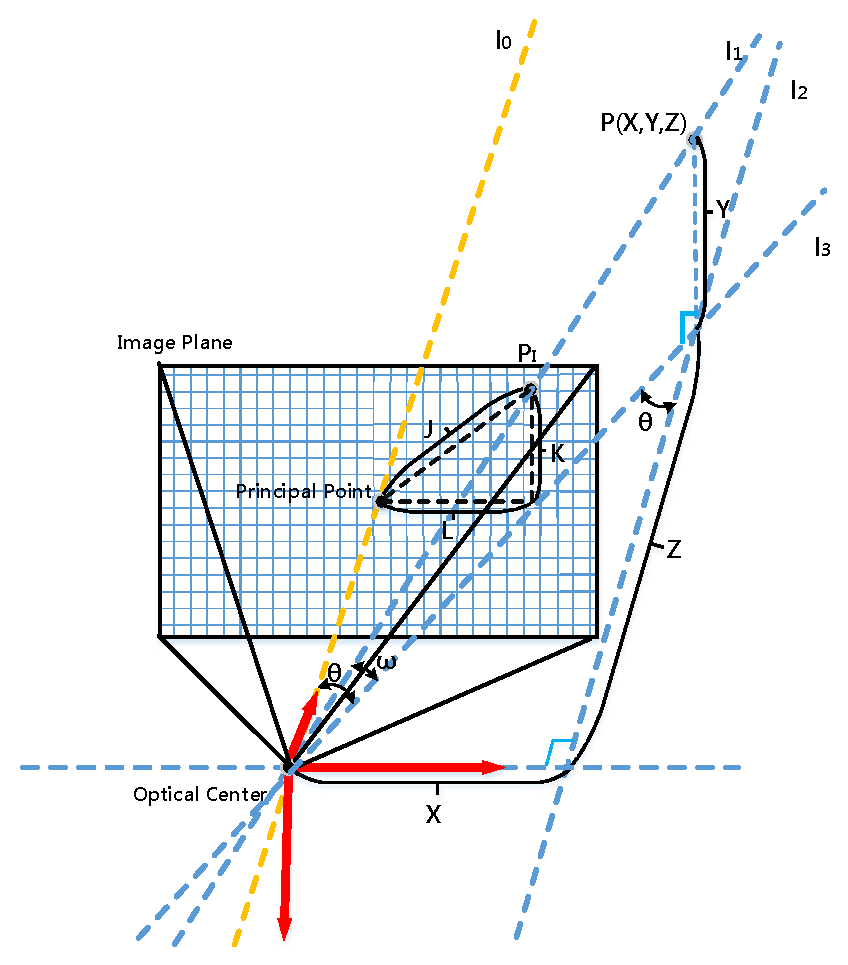
\includegraphics[width=2in, height=2in]{refgeo.eps}
\caption{Model of reference point geographical coordinates calculation.}
\label{fig_refgeo}
\end{figure}
Figure~\ref{fig_refgeo} shows the geometry model of reference point geographical coordinates calculation. As we figure out the depth Z of reference point P, we are able to calculate the coordinate $X$ and $Y$ of $P$.
\begin{equation}
    X=Z\cdot tan{\theta}
\end{equation}
where $\theta$ is the angle between $l_0$ and $l_3$, it is also as wide as the angle between $l_3$ and $l_2$. $\theta$ is proportional to $L$, which is horizontal component of pixel distance J from $P_I$ to the principal point, $P_I$ is perspective projection of point P on the image plane. The view angle $\alpha$ of camera is usually constant, so
\begin{equation}
    \theta = \frac{L\cdot \alpha}{w_{photo}}
\end{equation}
where $w_{photo}$ is the width of the photo in pixel.
Similarly, we can calculate the angle $\omega$ which is between $l_3$ and $l_2$. According to the height of optical center $h_{oc}$, we figure out
\begin{equation}
    Y=h_{oc}\pm (\sqrt{X^2+Z^2}\cdot tan{\omega} )
\end{equation}
which takes a plus sign when $P_I$ is above the principal point, minus sign when beneath.
\subsection{Reference Points Filtering}
High redundance of reference points is prone to incur high storage and search overhead. Additionally, indistinctive reference points may lead to error localization results. Therefore, it is necessary to filter the reference points to retain the most distinctive ones while ensuring the selected reference points evenly distributed in the indoor environment with desired density for localization.

To address this issue, we present an iterative filtering scheme. At the very beginning, all reference points are partitioned into different clusters according to their feature descriptors. Then reference points within each cluster are ordered by their \emph{neighbor density}, defined as the number of neighbors of one reference point with spacial distance less than $r$.

In each iteration, we select the largest cluster and check the reference point with the highest neighbor density.
Then the neighbor densities of reference points in the cluster are updated as well as their orders. If the neighbor densities of all points in a cluster are all lower than the the pre-specified threshold $D_{min}$, this cluster is marked as \emph{done} and will not be processed in the next iteration.
The above operations repeat until all clusters are marked as \emph{done}.

%Then we discuss the setting of parameters $r$, $D_{min}$.
As is shown in Figure~\ref{fig_site-survey}(c), the user can recognize both reference points $R_1$ and $R_2$ while standing in the shadow area. As is discussed in prior subsection, the angle $\eta$ and $\theta$ are within the range of $[\frac{\beta}{2}, \beta]$, thus the distance between $R_1$ and $R_2$ which is calculated as $d \cdot (\tan{\eta} + \tan{\theta})$ is within the range of $[d \cdot \tan{\beta}, 2 \cdot d \cdot \tan{\beta}]$. Here we assume that users will stand 2 meters away from the building structures at most of the times, thus $d \leq 2$. Then the distance between $R_1$ and $R_2$ should be less than $d \cdot \tan{\beta} = \frac{2}{\sqrt{3}}$. We need at least three reference points to inversely localize the user which will be discussed in following sections, so we require that at least one reference point exists between $R_1$ and $R_2$. To satisfy this condition, the distance from one reference point to its nearest neighbor should be less than $\frac{d}{2} \cdot \tan{\beta} = \frac{1}{\sqrt{3}}$. This setting is just a sufficient but not necessary condition for our localization scheme since users can change their view point to get more reference points. Then we set $r$ equal to $\frac{d}{2} \cdot \tan{\beta} = \frac{1}{\sqrt{3}}$ and $D_{min}$ equal to 1.



%\subsection{Feature skeleton construction}
%Design goal: easy site-survey, accurate feature skeleton, high quality feature filter.
%Steps:
%\begin{enumerate}
%\item Survey plan: given angle of view and floor plan how to survey.
%\item Skeleton construction: projecting features to floor plan.
%\item Feature filter: filter ''good'' features considering their quality and distribution.
%\end{enumerate}

%\subsection{Feature plane of view extraction}
%Design goal: high quality feature filter.

%Feature filter:
%\begin{enumerate}
%\item Remove noisy features from dynamic objects.
%\item Consistence with skeleton filter.
%\item Reduce communication cost by reducing the weight of centrol features. (Features near boundary are significant)
%\end{enumerate}

%\subsection{Automated Floor Plan Generation}
%\mynote{delete this section??}
%We build a coarse floor-plan from the reference points extracted in the site-survey stage.
%Reference points are grouped to different floors according to their attitudes. In each floor, the reference points are projected to plane based on their latitude and longitude. We then partition the plane into grids, the grid size is determined by the resolution of maps that we need. We regard each grid as a pixel and fill each grid with an intensity proportional to the number of reference points located in the grid.
%Thus we get an intensity image. We apply the state-of-the-art contour detection \mynote{cite a paper,figure} technique on the image to find the contour and by this way, we obtain an approximation of the floor-plan.




\section{Search Scheme}
\label{sec:search}
This section describes the reference point search scheme, which matches query feature points to reference points for the purpose of acquiring the nearest neighbors. We transform the matching problem to the well-known Nearest Neighbor (NN) search problem.
%The best candidate match for each feature point is found by identifying its NN in the database of reference points.
The distance between two feature points equals the Euclidean distance of their descriptors.
We also use this distance to measure the similarity of a match between query point and reference point and that a match has short distance means a good match with high similarity, and vice versa.
% We will eliminate the matches with low similarity by comparing the distance between query point and its closest neighbor to the distance between query point and its second-closest neighbor. The insights under the scheme lies in that correct matches should have the closest neighbor significantly closer than the closest incorrect match to achieve good matching. In the work of Lowe \cite{lowe2004distinctive}, by removing matches where the distance ratio between the closet and second-closet neighbors is greater than 0.8, it eliminates 90$\%$ of the false matches while discarding less than 5$\%$ of the correct matches.

In fact, exhaustive search for the NN in a large database is costly for both space and time. Many data organization and search schemes has been proposed to speed up the process, we propose a fast two-stage search scheme based on cluster \cite{gudmundsson2010large}. Both the visible orientation and feature descriptor of the point are considered in our method. Our two-stage search scheme includes preprocessing stage and search stage.
%The viewing angle of user's smart phone need to lie in the range of visible orientation of the found reference points. Meanwhile, the distance between feature descriptors of input feature points and reference points in database should be minimized.
\subsection{Preprocessing Stage}
In the preprocessing stage, we firstly partition all reference points into $b$ bins according to their visible orientation. Though reference point may be replicated in bins that overlap with its visible orientation, we just search the NN of the query feature point in only one bin according to its shooting angle.
\begin{algorithm}[!ht]
\caption{Clustering Descriptors}\label{clustering}
\begin{algorithmic}[1]
\Require reference point set $S$,set size $N$
\Ensure representative set $R$, cluster hash map $C\langle Representative,Cluster\rangle$
%\Function {Clustering}{$S,N$}
    \State $R \gets null$, $C \gets null$
    \While{$ |R| < \sqrt{N}$}
        \State Randomly choose a reference point $d$ from $S$
        \If {$d \notin R$}
            \State $R \gets R \cup d$
        \Else
            \State continue
        \EndIf
    \EndWhile
    \ForAll {$r \in R$}
        \State $w \gets \phi$
        \State $C.put(r,w)$
    \EndFor
    \ForAll {$d \in S$}
        \State $f \gets $ the cluster whose representative is closest to $d$
        \State $f.add(d)$
    \EndFor
    \State \Return $C, R$
%\EndFunction
%\Function {FindClosestCluster}{$d, R, C$}
%    \State $minDis \gets MAXDISTANCE$
%    \State $f \gets null$
%    \ForAll {$r \in R$}
%        \State $dist \gets distance(d,r)$
%        \If {$dist < minDis$}
%            \State $minDis \gets dist$
%            \State $f \gets C.get(r)$
%        \EndIf
%    \EndFor
%    \State \Return $f$
%\EndFunction
\end{algorithmic}
\end{algorithm}
In each bin, we randomly choose $\sqrt{N}$ reference points as the representatives of clusters. Then we put every reference point into the cluster whose representative is the closest to it. At last, we acquire $\sqrt{N}$ clusters, each of which has a unique representative. The cluster algorithm is described in Algorithm~\ref{clustering}.

For parameter $b$ we make a tradeoff between the space and the search time.
%The bins act as filters that prune significant portion of unmatched reference points according to their visible orientation at the cost of replications.
As $b$ increases, more bins are introduced and the angle range of each bin decreases. Thus the visible orientation of each reference point will span more bins and have more replications. Since the angle range of each bin gets wider, the number of reference points in each bin decreases, the search time decreases as well. Without loss of generality, we set $b$ equal to 30 degree.

\subsection{Search Stage}
In the search stage, in order to find descriptor $Q$'s nearest neighbors in its visible orientation bin, we propose a 2-round search algorithm. In the first round, we calculate the distance between $Q$ and each representative. We denote the closest representative as $T$.
%\begin{algorithm}[!ht]
%\caption{K Nearest Neighbor Searching }\label{searching}
%\begin{algorithmic}[1]
%\Require feature descriptor $Q$, representative set $R$, cluster hash map $C\langle Representative,Cluster\rangle$
%\Ensure K nearest neighbor feature descriptor set T
%%\Function{Searching}{$Q, C, R$}
%    \State $f \gets  $the cluster whose representative is closest to $Q$
%    \State $T \gets \phi$
%    \ForAll {$d \in f$}
%        \State $t \gets $the point in $T$ with maximum distance to $Q$
%        \If {$distance(Q,d) < distance(Q, t)$}
%            \State $T \gets T - t$
%            \State $T \gets T \cup d$
%        \EndIf
%    \EndFor
%   \State \Return $T$
%%\EndFunction
%\end{algorithmic}
%\end{algorithm}
It is supposed $Q$'s NN belongs to $T$'s cluster. Therefore, we look for $Q$'s NN in $T$'s cluster in the second round. We compute the distances between $Q$ and each feature point in $T$'s cluster. Finally, we obtain $K$ closest feature points as $Q$'s top-K NN.
%The search algorithm is described in Algorithm~\ref{searching}.
\subsection{Complexity Analysis}
\label{complexity}
In the preprocessing stage, assume there are $b$ bins and each bin has $N$ reference points averagely. With respect to one bin, we will compare $N$ reference points to $\sqrt{N}$ representatives, \ie we will do $b\times N\times \sqrt{N}$ comparisons in all. At query time, we compare the query feature descriptor $Q$ to representatives in the specific bin determined by the orientation of user's camera. $Q$ is firstly compared to $\sqrt{N}$ representatives to find the nearest cluster $f$. Then $Q$ is compared to each reference point in $f$. On average, each cluster contains $\sqrt{N}$ reference points. Thus, for one query feature point $Q$, we need to do a total of $2\sqrt{N}$ comparisons.


\section{Inverse Localization}
\label{sec:inverse}

\subsection{Location Determination Problem}
In this section, we form our localization problem as the Location Determination Problem (LDP)\cite{fischler1981random}. The definition of a traditional LDP problem is as follows. Given a photo depicting a set of $n$ reference points with known locations, we determine the geographical coordinates of the place where the photo was taken. It has been proved that when $n$ equals to 3, the the problem can be solved\cite{fischler1981random}. We derive the orientation of camera with onboard sensors of the smart phone which helps to facilitate the localization process.
\begin{figure}[!ht]
\centering
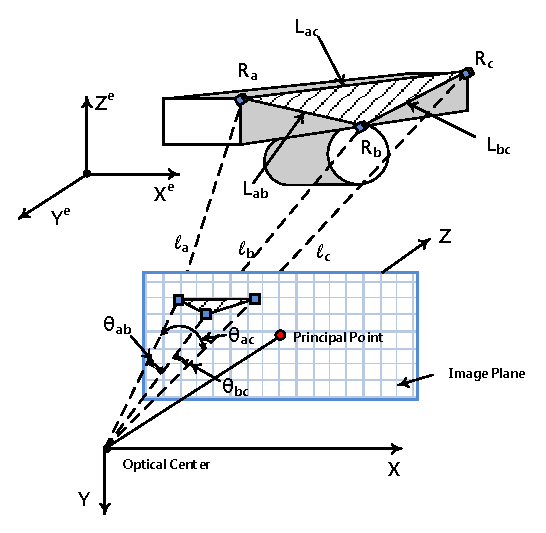
\includegraphics[width=1\linewidth, height=1.6in, clip,keepaspectratio]{ldp2cc.eps}
\caption{Determination of the location of user based on reference points.}\label{fig_ldp}
\end{figure}
We assume that the optical axis of the camera pierces the image plane on the \emph{principal point} and the \emph{focal length} of the camera is known.
As shown in Figure~\ref{fig_ldp}, the user takes a photo of the scene in front of him/her and three references points, namely, $R_a(X_a, Y_a, Z_a)$, $R_b(X_b, Y_b, Z_b)$ and $R_c(X_c, Y_c, Z_c)$ are projected to the image plane.
Through the reference point search scheme, we have obtained the correspondences between image points and reference points.
According to the distance from the image point projected by $R_a$ to the the point projected by $R_b$, we can easily derive $\theta_{ab}$, the angle between the line from the \emph{optical center} to $R_a$ and the line from the \emph{optical center} to $R_b$. We can also derive $\theta_{bc}$ and $\theta_{ac}$ in the same way.
%It has been proved that known the distances from three reference points to the \emph{optical center}, the location of the \emph{optical center} can be solved\cite{fischler1981random}.
% Thus the LDP problem can be transformed to the problem of calculating the distances from $n$ reference points to the optical center given locations of $n$ reference points as well as the angles from the optical center to each pair of reference points.
Let $L_{ab}$, $L_{bc}$ and $L_{ac}$ denote the distances between three reference points respectively, and $l_a$, $l_b$, $l_c$ denote the distances from each reference point to the \emph{optical center}.
We have the following equation group according to the law of cosine:
\begin{equation}
\label{equations}
\left\{
\begin{array}{l}
(L_{ab})^2 = (l_a)^2 + (l_b)^2 - 2 l_a\cdot l_b\cdot \cos(\theta_{ab})  \\
(L_{bc})^2 = (l_b)^2 + (l_c)^2 - 2 l_b\cdot l_c\cdot \cos(\theta_{bc}) \\
(L_{ac})^2 = (l_a)^2 + (l_c)^2 - 2 l_a\cdot l_c\cdot \cos(\theta_{ac})
\end{array}
\right.
\end{equation}
The above equation group may have multiple solutions,
%and after removing the geometrically isomorphic negative solutions, there are 4 solutions left.
we make use of the technique proposed in \cite{fischler1981random} to solve it and use the orientation of the camera to eliminate infeasible solutions. Every solution includes distances from three reference points to the \emph{optical center}.

We use the distance between query feature point and its nearest neighbor of reference point to measure the similarity of the match mentioned before. Each time, we select three matches with the highest similarity from the result set $T$ of that searching stage to form a trine.

Based on the solution of equation group~\ref{equations}, we are able to figure out the geographical location of the \emph{optical center} $CP(X,Y,Z)$, \ie user's geographical location, by solving another equation group~\ref{cp_equations}.
\begin{equation}
\label{cp_equations}
\left\{
\begin{array}{l}
\sqrt{(X-X_a)^2+(Y-Y_a)^2+(Z-Z_a)^2} = l_a  \\
\sqrt{(X-X_b)^2+(Y-Y_b)^2+(Z-Z_b)^2} = l_b \\
\sqrt{(X-X_c)^2+(Y-Y_c)^2+(Z-Z_c)^2} = l_c
\end{array}
\right.
\end{equation}
Equation group~\ref{cp_equations} describes the distances from $CP$ to three reference points. This equation group may have multiple solutions as well. Every solution will be treated without distinction to estimate its error.

We take the concept of "consensus" proposed by \cite{fischler1981random} to estimate error of each solution. With respect to the solution $S_0$, one reference point $r$ from $T$ reaches a consensus with $S_0$ if $r$ passes the estimate check function $Func$. $Func$ can be designed in a variety of forms. Our estimate check function $Func1$ is designed as follows: $Func1$ computes reference point $r$'s pixel coordinates in the picture which takes $S_0$ as the optical center. If the distance between $r$'s newly computed coordinates and its original coordinates does not exceed threshold $t$, then $r$ reaches a consensus with $S_0$. We put reference points which reach consensus with $S_0$ into consensus set $C_{S_0}$. If the ratio $\frac{|C_{S_0}|}{|T|}$ exceeds the threshold $w$, then $S_0$ will be considered as one candidate solution and added to set $F$. After every solution has been processed, we are able to figure out the final result of CP's location from set $F$ by selecting the candidate with highest consensus.
\subsection{Optimization of Estimate Check Function}
Aiming at enhancing localization performance of $Func1$, we refine it to form another estimate check function $Func2$ by appending a post-process after $Func1$. When we obtain $F$, rather than taking the candidate with highest consensus as the final result, we select the candidate through the vote. For one candidate $c$, a reference point $r$ in $T$ will vote for $c$ if the distance from $r$ to $c$ is not longer than threshold $d_{th}$. We discard the candidates with fewer votes and keep $K$ candidates with more votes. From these $K$ candidates, we pick the one derived from the trine whose triangle area is the largest among them as the final result.

$Func2$'s post-process is inspired by this phenomena: if three reference points in one trine are close to each other, then the solution of Equation group~\ref{equations} is more prone to error. If a trine has a larger area, the distances between three reference points in it are comparatively longer, which reduces the chance of error prone.

%When more reference points are observed, we compute the location of a user with different group of reference points and conduct an integrated optimization process to eliminate errors.
%In this work, we apply the Random Sample Consensus (RANSAC) \cite{fischler1981random} in our approach.
%RANSAC is an efficient method for fitting a model to experimental data. At the very beginning, it randomly select a minimum set of data points $S_1$ to instantiate the model $M_1$. Then RANSAC use $M_1$ to find the subset $S^c$ of data that are within some error bound. The subset is referred to as the \emph{consensus set} of $S_1$. If the number of $S^c$ is above some threshold, use $S^c$ to compute a new model. Otherwise, we select a new initiate set $S_2$ and repeat the above operations. This process ends after a number of rounds, we solve the problem with the largest consensus set. \mynote{check in paper}
%Our inverse localization scheme takes three types of inputs.

%\begin{enumerate}
%\item 1) A set of 5-tuples each of which includes the 3-D coordinates in earth coordinate system of a reference point, the 2-D image plane coordinated of the associated image point.
%\item 2) The probability $\omega$ that a 5-tuples contains a gross error.
%\item 3)
%\end{enumerate}

%The integrated algorithm contains the following steps.

%\begin{enumerate}
%\item 1) Three 5-tuples are selected and form the initial set $S1$.
%\item 2) The location of the optical center and thus the user is calculated accordingly.
%\item 3) Perturbing the image plane coordinated.
%\item 4) Perturbing the image plane coordinated.
%\end{enumerate}


%
%
%\subsection{Trace-based Optimization}
%Although our perspective approach calculate user locations based on data fusion from multiple reference points in the largest consensus set, the result at single location would still deviate from the real value or exhibits ambiguities while working under indistinctive indoor environments.
%It is due to the occasional ambiguities in vision feature matching. To address the problem, we present a trace-based algorithm to optimize the localization results. As users walk in the indoor environment, the localization service continuously generates locations at different points according to vision features. Besides, we can track the movement vectors of users using onboard sensors of the smart phone.
%A series of consecutive movement vectors form a trace that can connect successive localization snapshots.
%Based on the movement trace of a user, we can eliminate ambiguities and recover missing points by interpolation for the localization results.
%As shown in Figure~\ref{fig_trace}, for each pair of neighboring locations, we compute the similarity between the move vector and distance vector of the two locations. If the similarity of the two vectors are above a pre-specified threshold, these two locations are grouped into one component. Two adjacent components can merge to one. By this way, we find outliers among the locations. In the example of Figure~\ref{fig_trace}, with the movement vector, we can easily distinguish the correct location from the wrong ones.
%\begin{figure}[t!]
%\centering
%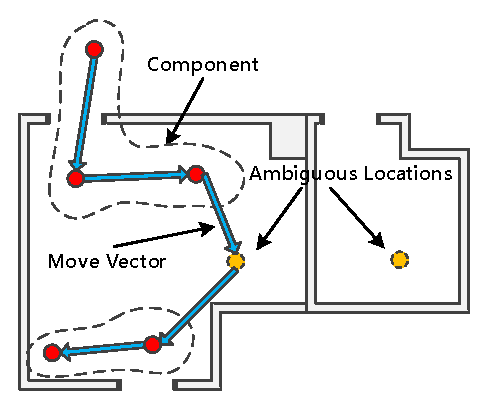
\includegraphics[width=1\linewidth, clip,keepaspectratio]{trace2.eps}
%\caption{Trace-based Optimization.}\label{fig_trace}
%\end{figure}
%Besides, the movement trace can also help us to recover missing coordinates by interpolation for the localization results.
%
%
%To obtain the moving vector of users, we apply one of the recent method proposed in Montage \cite{zhang2014montage} which combines dead reckoning and the stride length based approach to estimate the moving distance and leverage the filtered horizontal accelerations along the east and north axes at the earth coordinate system to measure the moving orientation of each step.
%


%\section{Trace Optimization}
%\label{sec:trace}
%\input{trace.tex}

\section{Implementation and Evaluation}
\label{sec:eva}
\subsection{System Implementation}
We have implemented \oursystem both on Android smartphone and laptop. The user application is implemented on HTC NEW ONE X with azimuth sensor and WiFi , as well as the site-survey tool application. The server side of \oursystem is implemented on ASUS A43S laptop installed Win7 with four 2.20GHz Intel Core i7 processors, 8GB of DDR2-memory.

For the software part of client application, the code for feature extractor module is implemented using C++ and OpenCV library for Android, the remaining parts are implemented in JAVA , the client application runs on the Android Operating System. The site-survey tool application also runs on Android platform. The server side is implemented using C++ and JAVA.
%It is supposed that both server and client access to the same local area network so that they can communicate with each other.
\subsection{Case Study \uppercase\expandafter{\romannumeral1}: Office Environment}
\subsubsection{Site Survey in Office Environment}

As we have the floor plan of the experimental office environment with $60m \times 28m$ area, we annotate each shooting point on the floor plan with its relative geographical coordinates. Figure~\ref{office_site} shows the floor plan of the office, the yellow star is the original point of the office coordinate system, the red line marks the survey track and white dots mark the shooting points, the distance between every two adjacent shooting points is $1.6m$. On each shooting point, we will take pair-photos from two directions, if the shooting point is on the horizontal segment of green line we take photos from north and south, on the vertical segment we take photos from east and west.
\begin{figure}[h!]
\centering
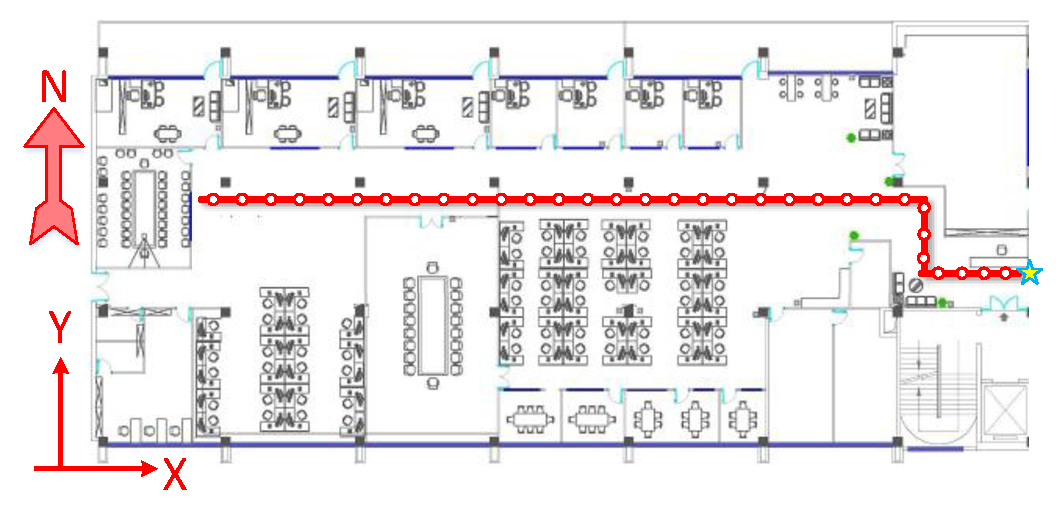
\includegraphics[width=1\linewidth, height=1in, clip,keepaspectratio]{officesite.eps}
\caption{Site survey track in office.}\label{office_site}
\end{figure}

After processing the photos and calculate the geographical locations of reference points, we are able to project the reference points denoted by red points on the floor plan as shown in Figure~\ref{office_ref}. We have filtered out some reference points, the remaining reference points are stable, \ie they are located on the building structure like walls, windows and so on.
\begin{figure}[!htbp]
\centering
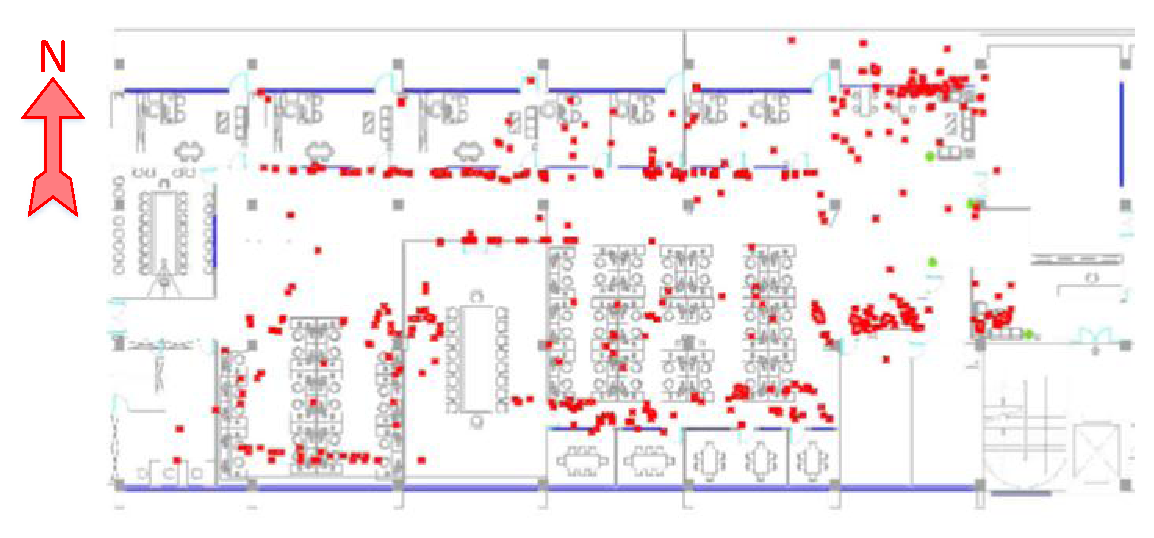
\includegraphics[width=1\linewidth, height=1.1in, clip,keepaspectratio]{officeref4.eps}
\caption{Project filtered reference points on floor plan.}\label{office_ref}
\end{figure}

\subsubsection{Impact of Reference Point Database Size}
In the stage of building up reference point database, the tighter parameters for reference points filtering the less reference points remain, thus we can obtain several reference point databases with different sizes by set different parameters. We study the clustering cost of time and space for a range of sizes of reference point database, Table~\ref{tab_office_cluster} shows the results. As analysed in section~\ref{complexity}, having more reference points results in a longer clustering process, more clusters and larger space, and conversely the less overhead in time and space.
\begin{table}[!htbp]
\centering
\begin{tabular}{ccccc}
\hline
ID &Ref points &Clusters &Time(ms) & \begin{minipage}{2cm}Average cluster size(KB) \end{minipage}\\
\hline
1 &2718 &52 &603 &31.9\\
2 &2088 &46 &371 &27.6\\
3 &1279 &36 &362 &21.75\\
4 &816 &29 &274 &17.3\\
\hline
\end{tabular}
\caption{\label{tab_office_cluster}Impact of reference point database size on clustering stage for office environment.}
\end{table}
\begin{figure*}
\centering
\subfigure[Average LE] {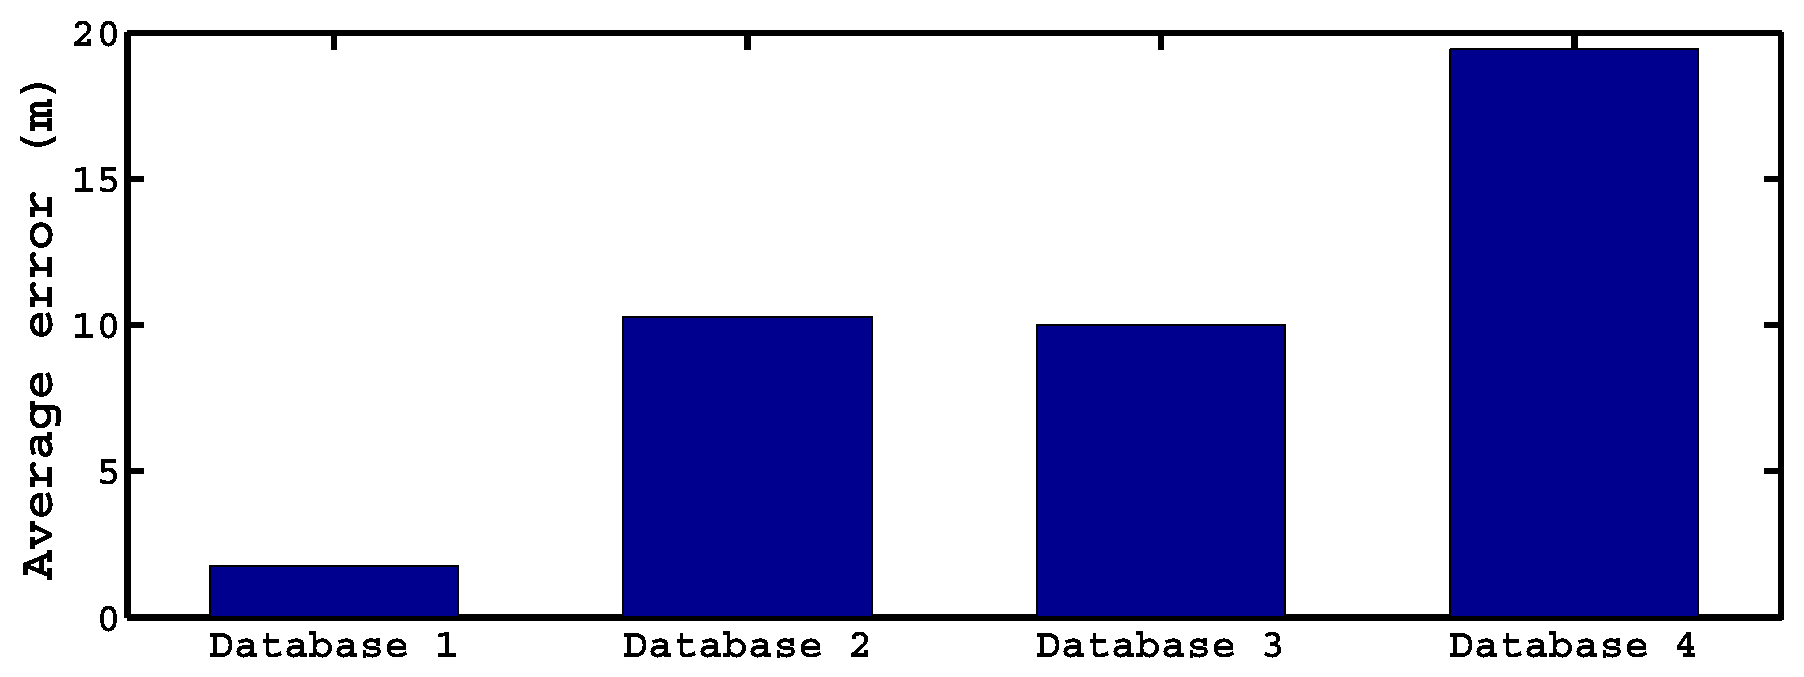
\includegraphics[width=1.7in, height=1.0in]{bar_office4ds.eps}}
\subfigure[CDF of LE] {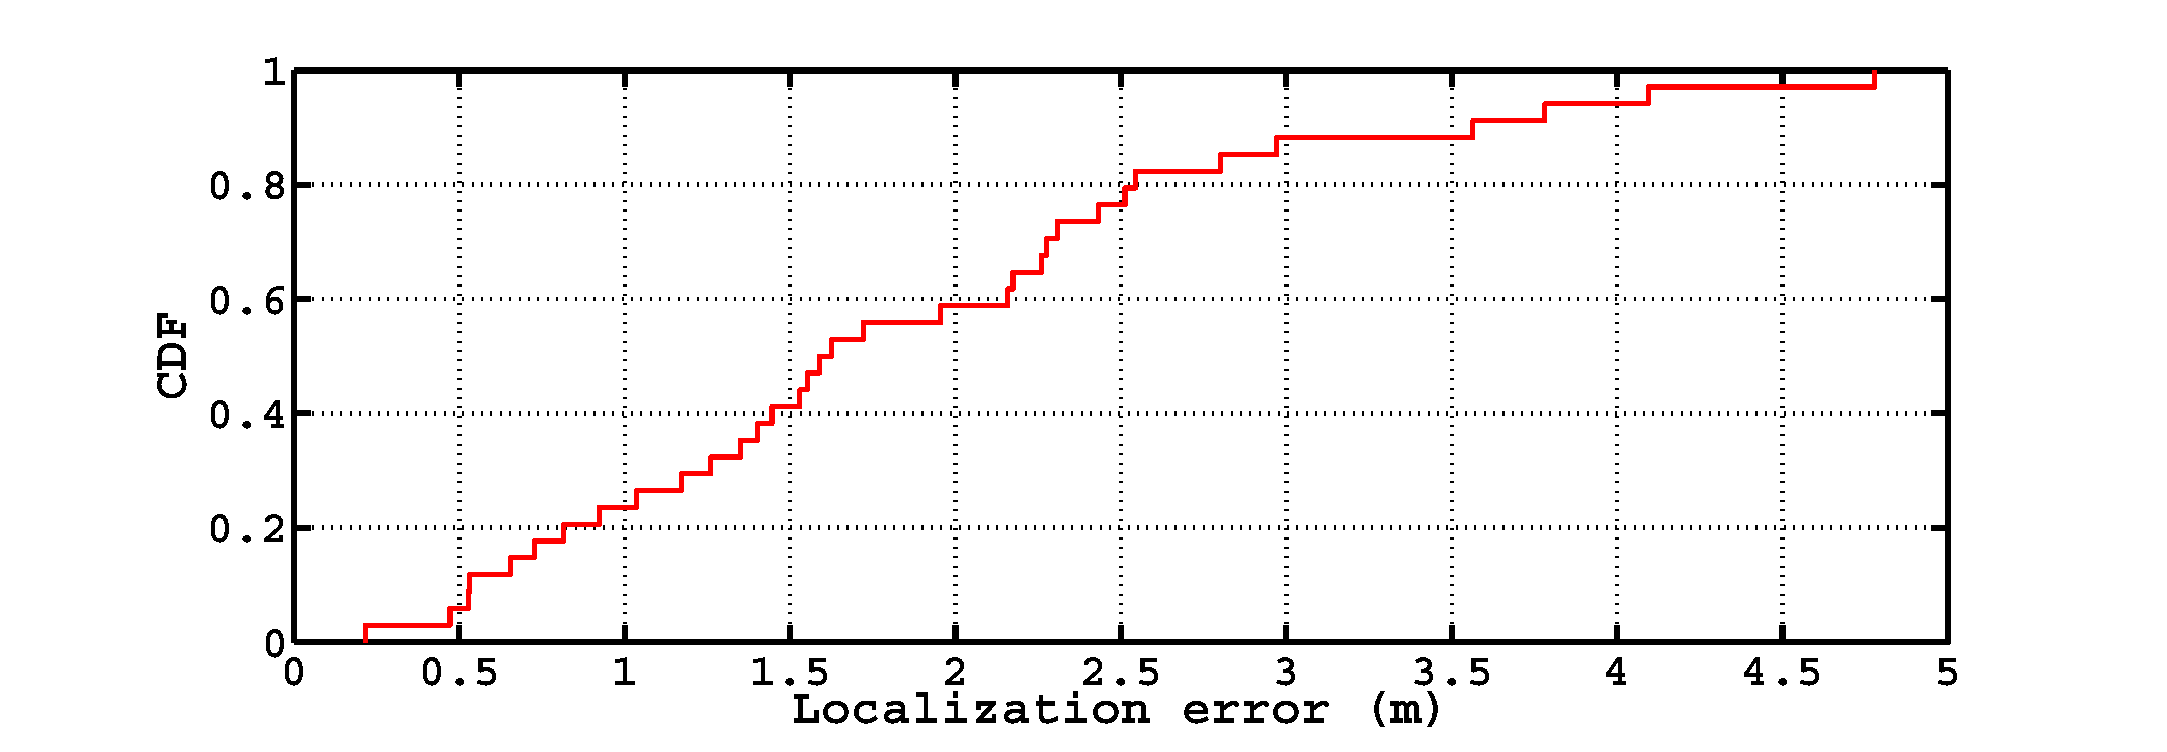
\includegraphics[width=1.7in, height=1.0in]{cdf_Office.eps}}
\subfigure[CDF of LT] {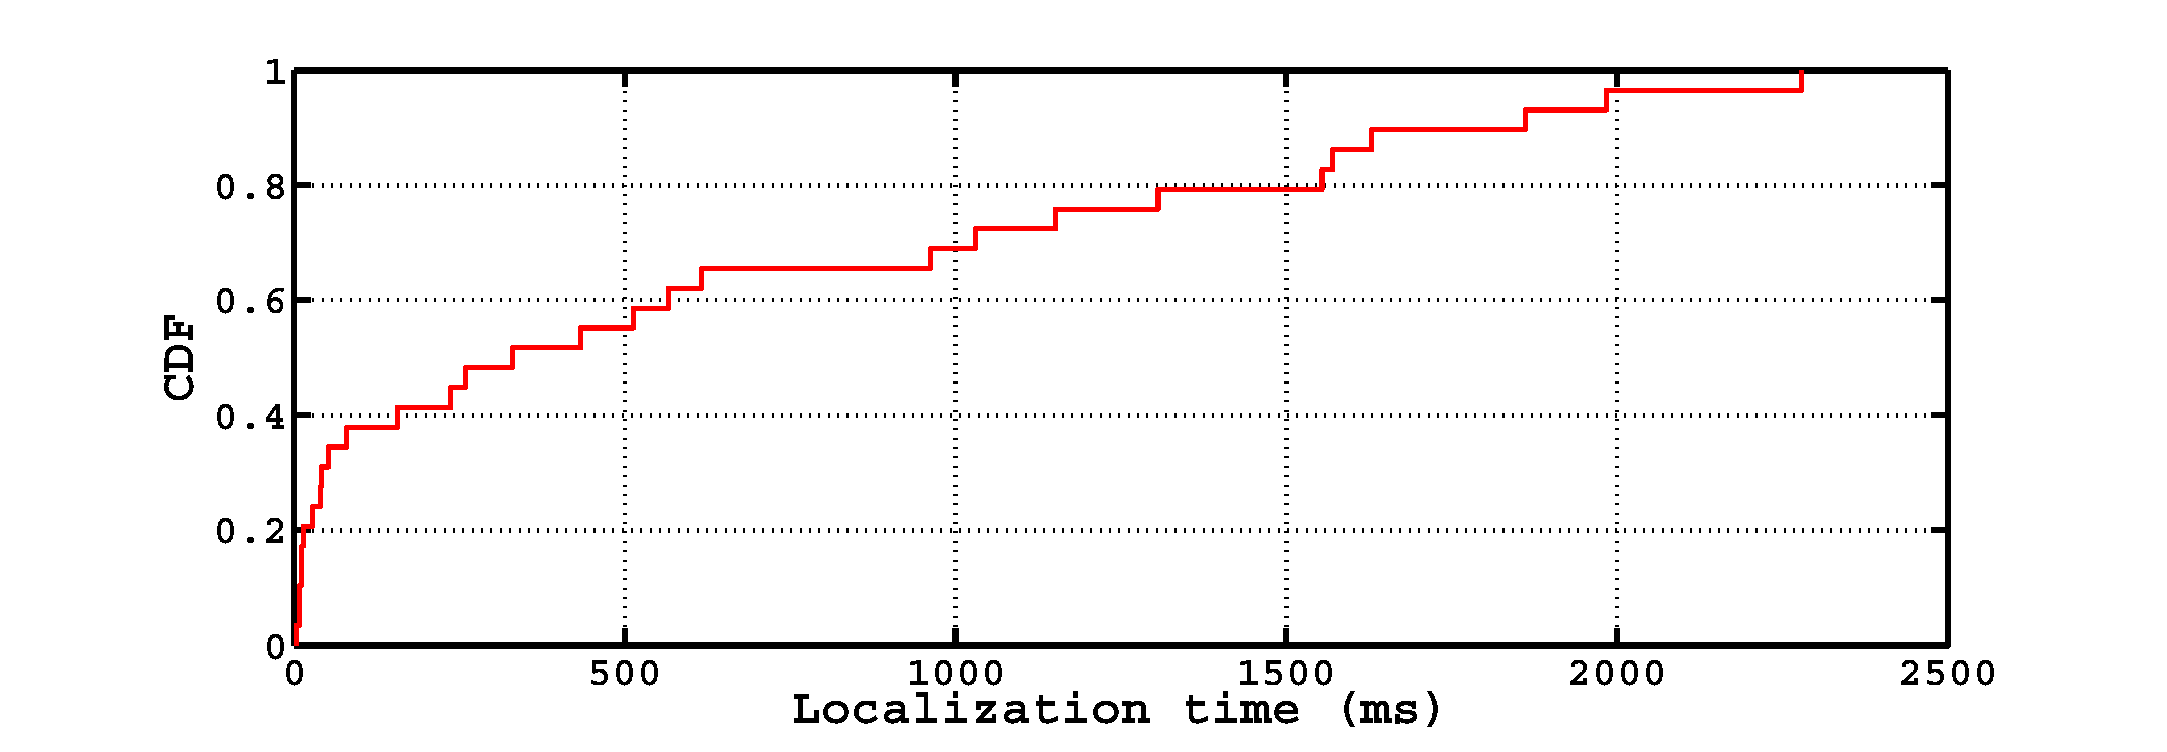
\includegraphics[width=1.7in, height=1.0in]{cdf_office_time.eps}}
\subfigure[CDF of LE] {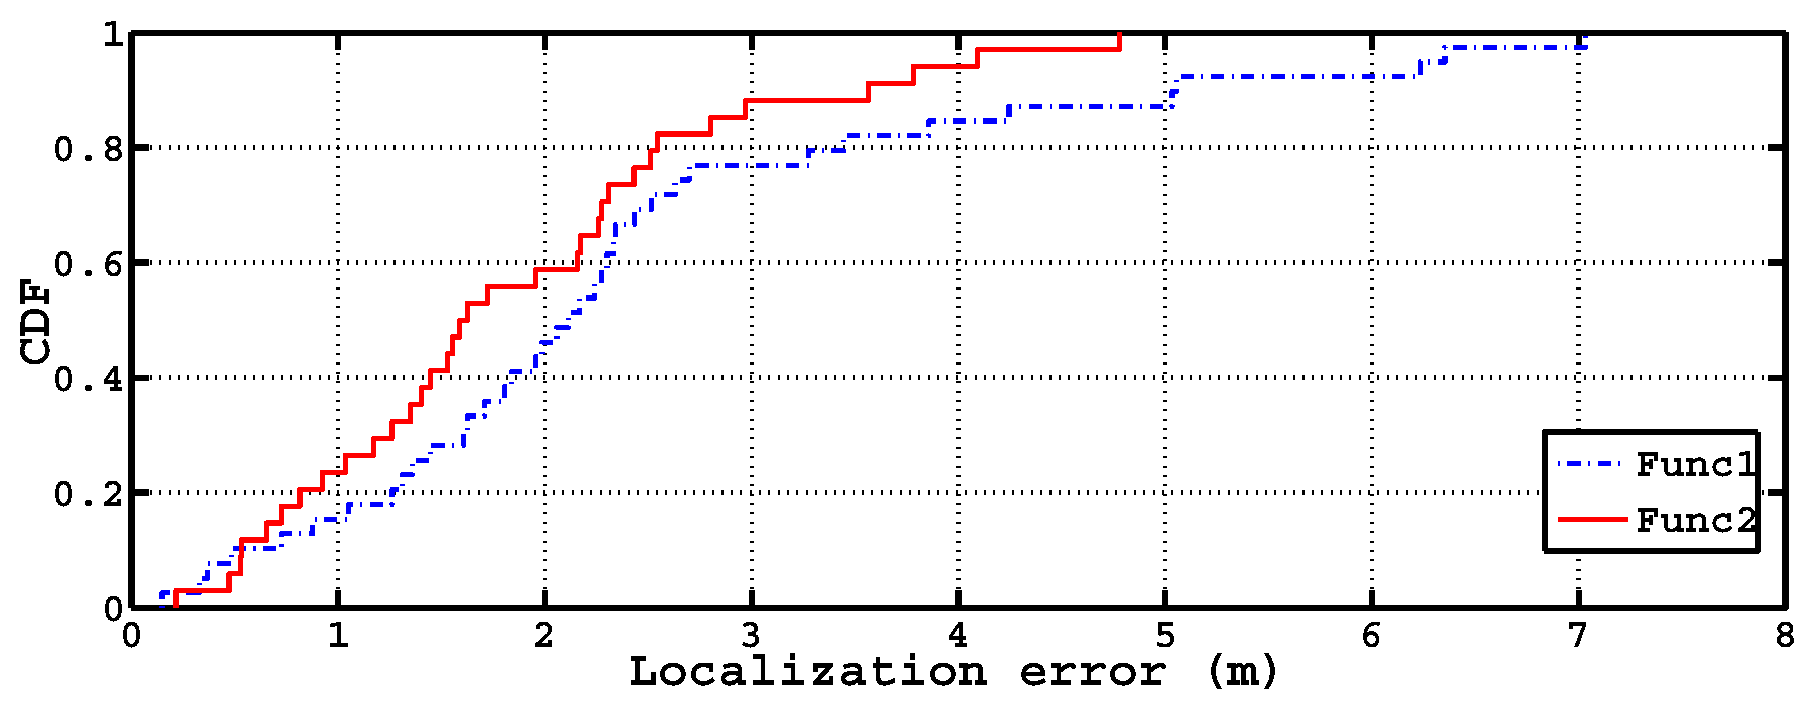
\includegraphics[width=1.7in, height=1.0in]{office_func12.eps}}
\caption{Localization performance in office environment reference database: (a)Average LE of 4 reference point databases. (b)CDF of LE run on database 1. (c)CDF of localization time on database 1.(d)CDF of LE for $Func1$ and $Func2$ in office environment.}
\label{ref_size}
\end{figure*}
Figure~\ref{ref_size}(a) shows the localization error(LE) run on four reference point databases of office environment. Obviously, database 1 which has the largest number of reference points achieves the lowest average error(AE) $1.76m$ among four databases. Database 4 which has the least number of reference points performs a low localization accuracy, its AE is $19.4m$. The AE of database 2 is $10.4m$ which is close to database 3. This result tells us that there is a tradeoff between overhead and localization accuracy, \ie the database with larger size will have more accurate localization results, however, create more overhead and the database with smaller size will cause less overhead but acquire worse localization results. Taking the office environment into account, we are convinced that the size of database for the building whose area is about $1600m^2$ should be almost 2000 reference points.

Figure~\ref{ref_size}(b) shows the CDF of the LE run on database 1. On database 1, we can locate the user with an accuracy of $1.58m$ for 50\% and  $3.56m$ for 91\%. Figure~\ref{ref_size}(c) shows the localization time(LT) run on four office reference point databases, the time of localization process is no more than $2.2s$. With respect to database 1, the localization time is $0.5s$ for 50\% and $1.5s$ for 90\%, which is fast enough to achieve real time localization.

%
%\begin{figure}[t]
%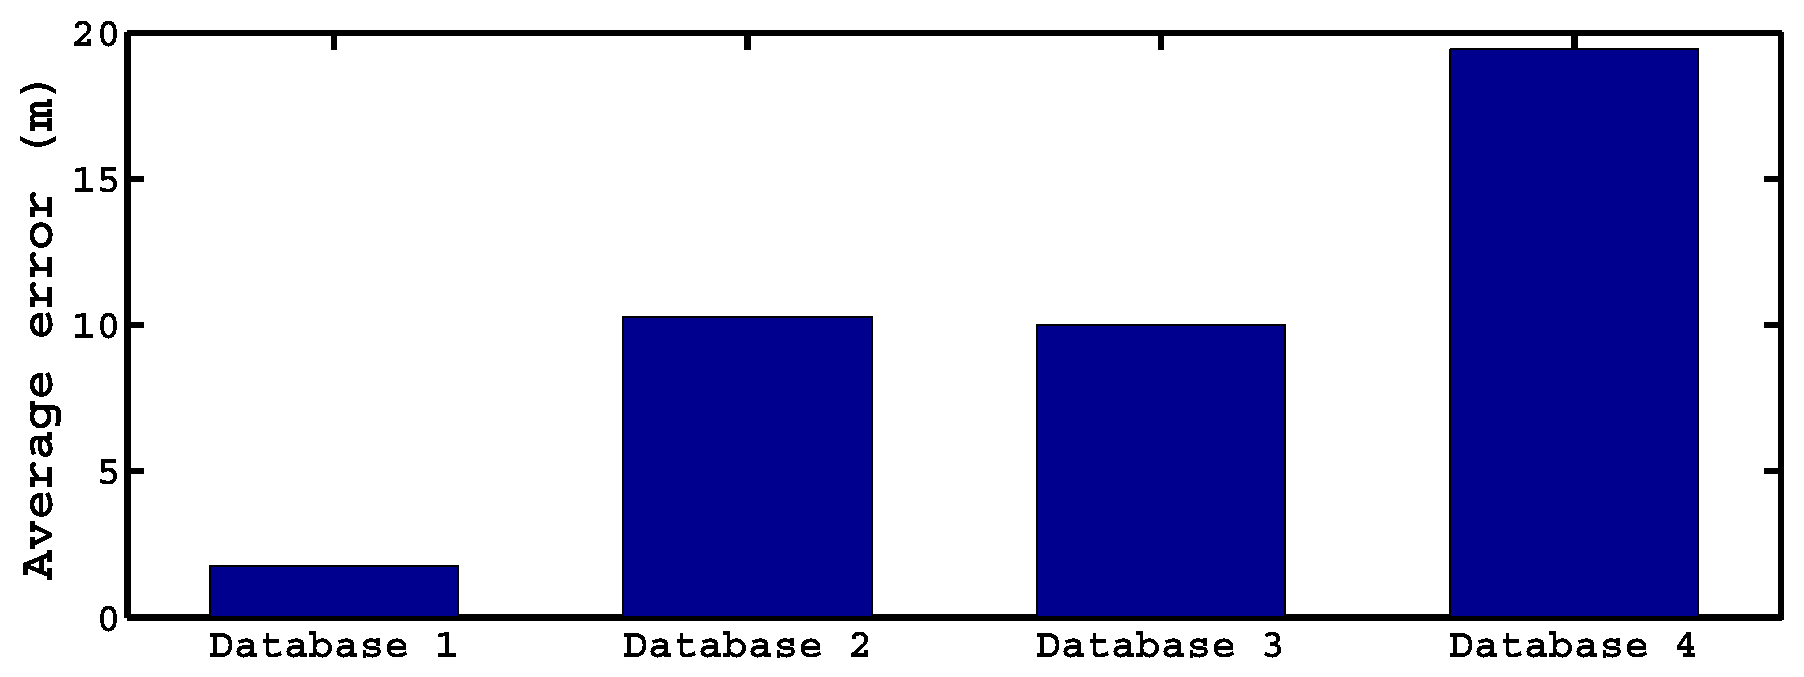
\includegraphics[width=1\linewidth, clip, keepaspectratio]{bar_office4ds.eps}
%\caption{Average LE of 4 reference point databases.}
%\label{bar_office}
%\end{figure}
%\begin{figure}[t!]
%\includegraphics[width=1\linewidth, clip, keepaspectratio]{cdf_office.eps}
%\caption{CDF of LE run on database 1.}
%\label{cdf_office}
%\end{figure}
%\begin{figure}[t!]
%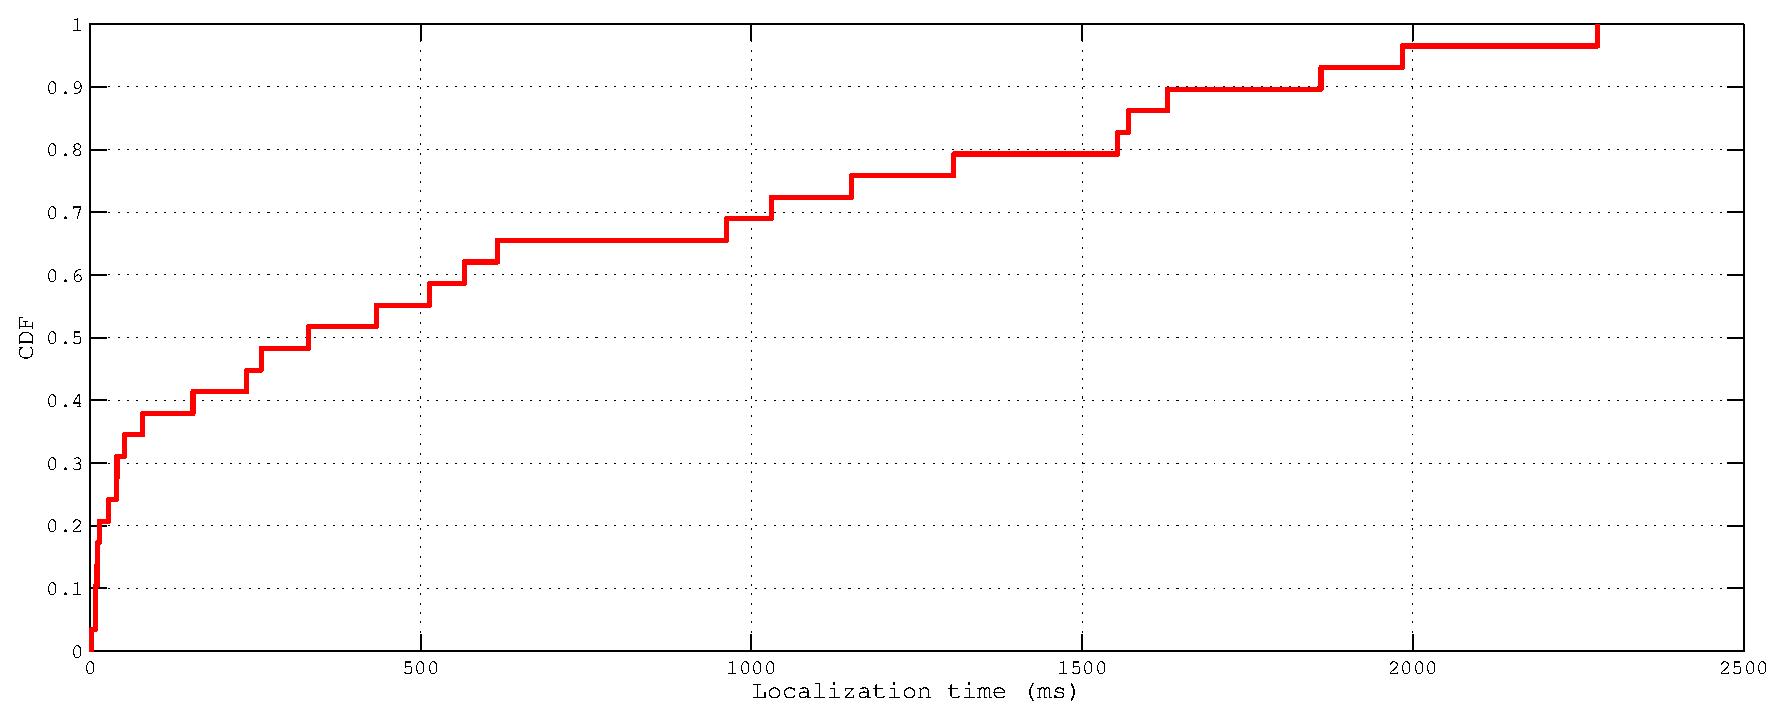
\includegraphics[width=1\linewidth, clip, keepaspectratio]{cdf_officetime.eps}
%\caption{CDF of localization time run on databases 1.}
%\label{cdf_officetime}
%\end{figure}
\subsubsection{Impact of Check Function $Func$}
%This section describes how the size of query point set affects the accuracy of localization. We randomly select $K$ feature point from one query point file to observe the changes of LE. According to the common sense, larger query set should reduce LE. While from Figure~\ref{bar_office_query}, we observe that the LE does not decrease as expected when query set size K increases. The reason for this phenomenon is that more query points may even cause more mismatches between query point and reference point which degenerates the localization accuracy. And LE reaches minimum values when K equals to 25\% or 50\%, which gives us a insight that we can save the communication cost of client by reducing query point set.
%\begin{figure}[t!]
%\centering
%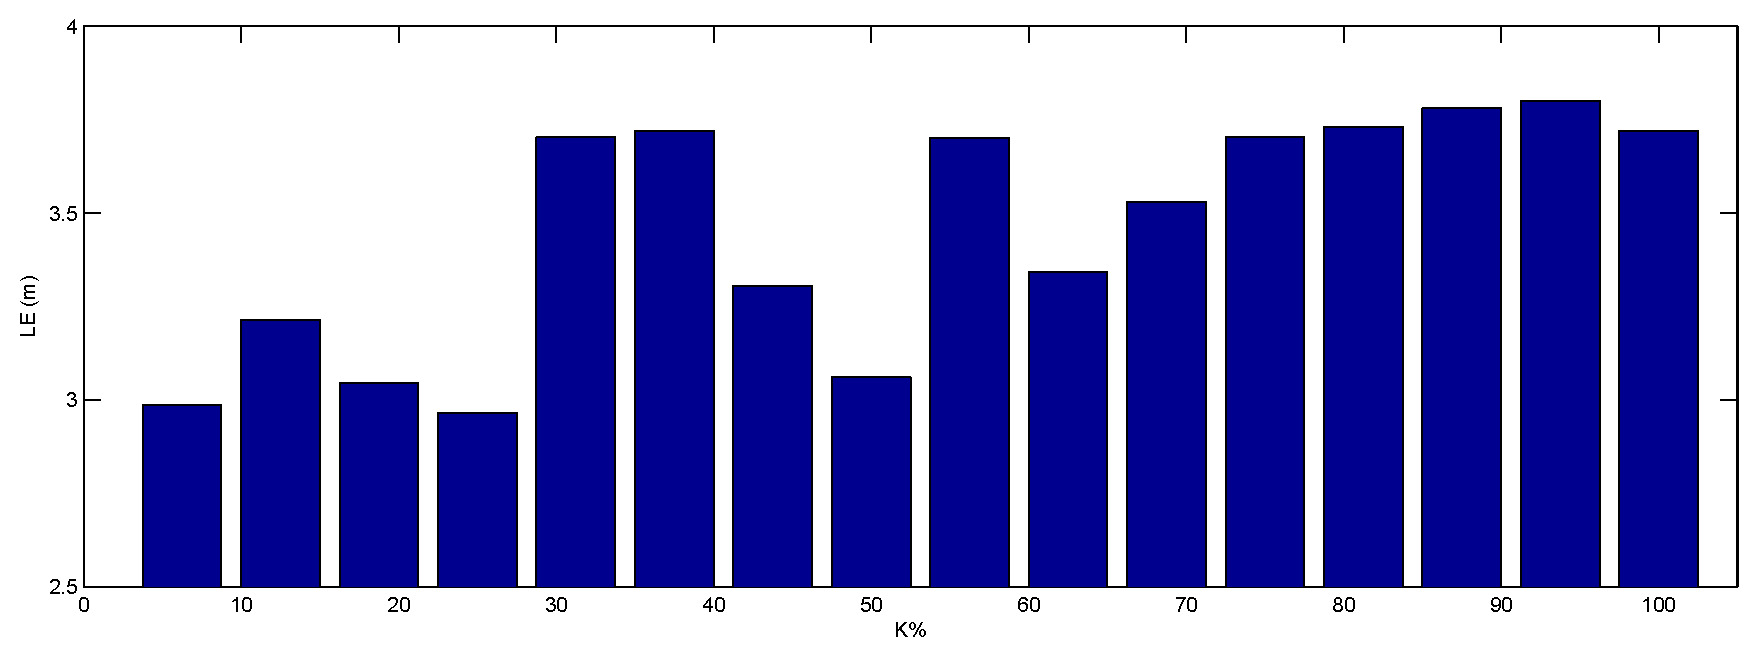
\includegraphics[width=1\linewidth, clip,keepaspectratio]{bar_officequeryK.eps}
%\caption{Average LE of K query feature points.}\label{bar_office_query}
%\end{figure}

%check function%
This section gives an inspection on how different check function $Func$ affect the performance of \oursystem. We use $Func_1$ and $Func_2$ respectively to make accuracy experiments on database 1, the results are shown in Figure~\ref{ref_size}(d). Compared to $Func1$ whose LE is $5.1m$ by 91\%, $Func2$ improves the localization accuracy notably, whose LE is $3.9m$ by 91\%.
%\begin{figure}[!tbp]
%\centering
%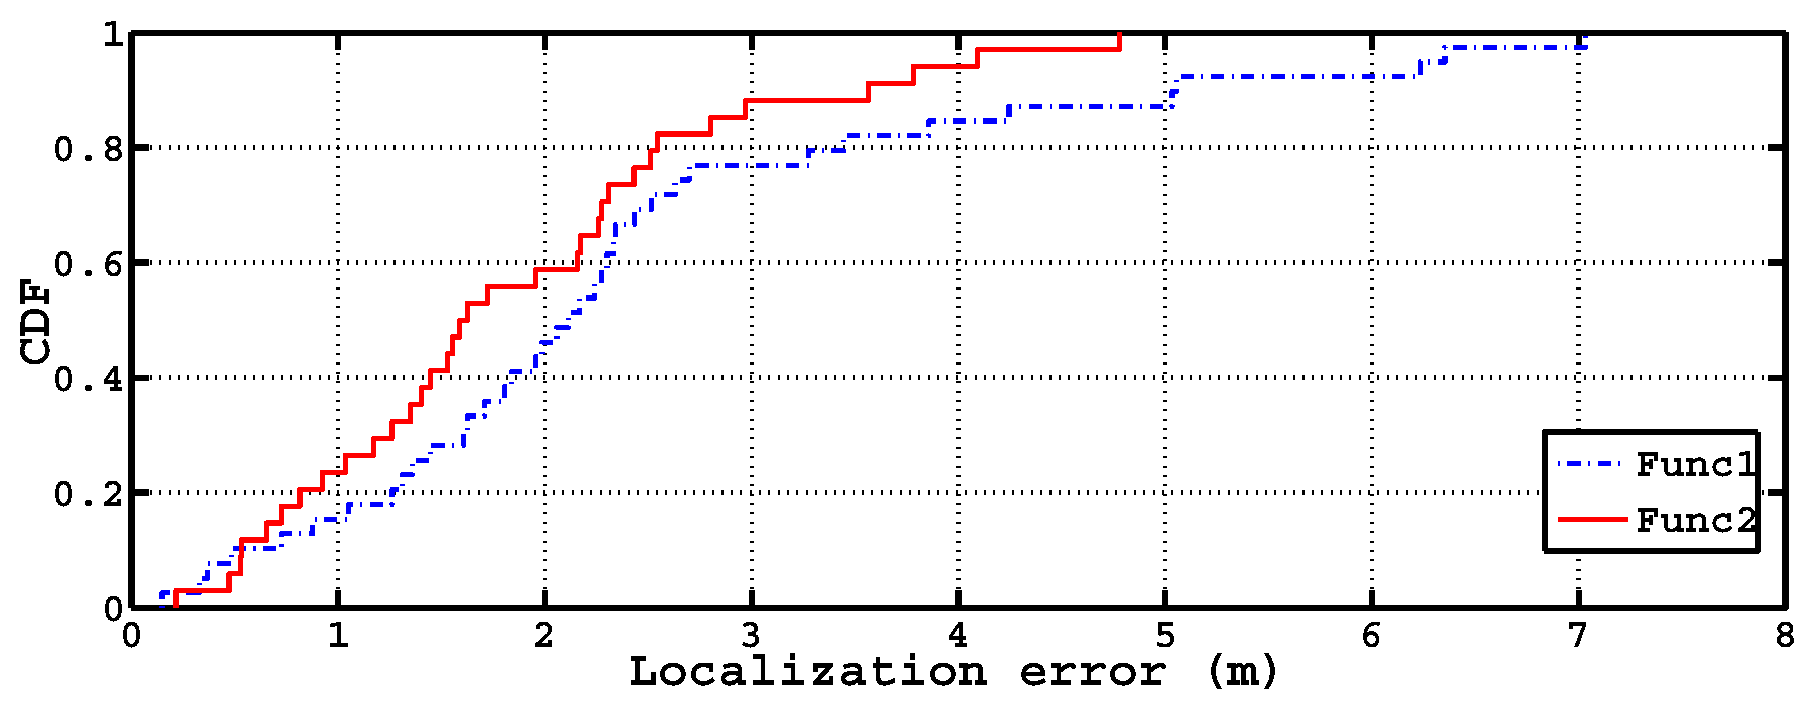
\includegraphics[width=2.2in,height=1.6in, clip,keepaspectratio]{office_func12.eps}
%\caption{CDF of LE for $Func1$ and $Func2$ in office environment.}\label{office_func12}
%\end{figure}
%\subsubsection{Impact of Consensus Estimate Parameters}
%The parameters for consensus estimate also affect the accuracy of \oursystem. Figure~\ref{office_para}(a) shows the AE for different $w$. Figure~\ref{office_para}(b) shows the AE for different $t$.
%\begin{figure}[!htbp]
%\centering
%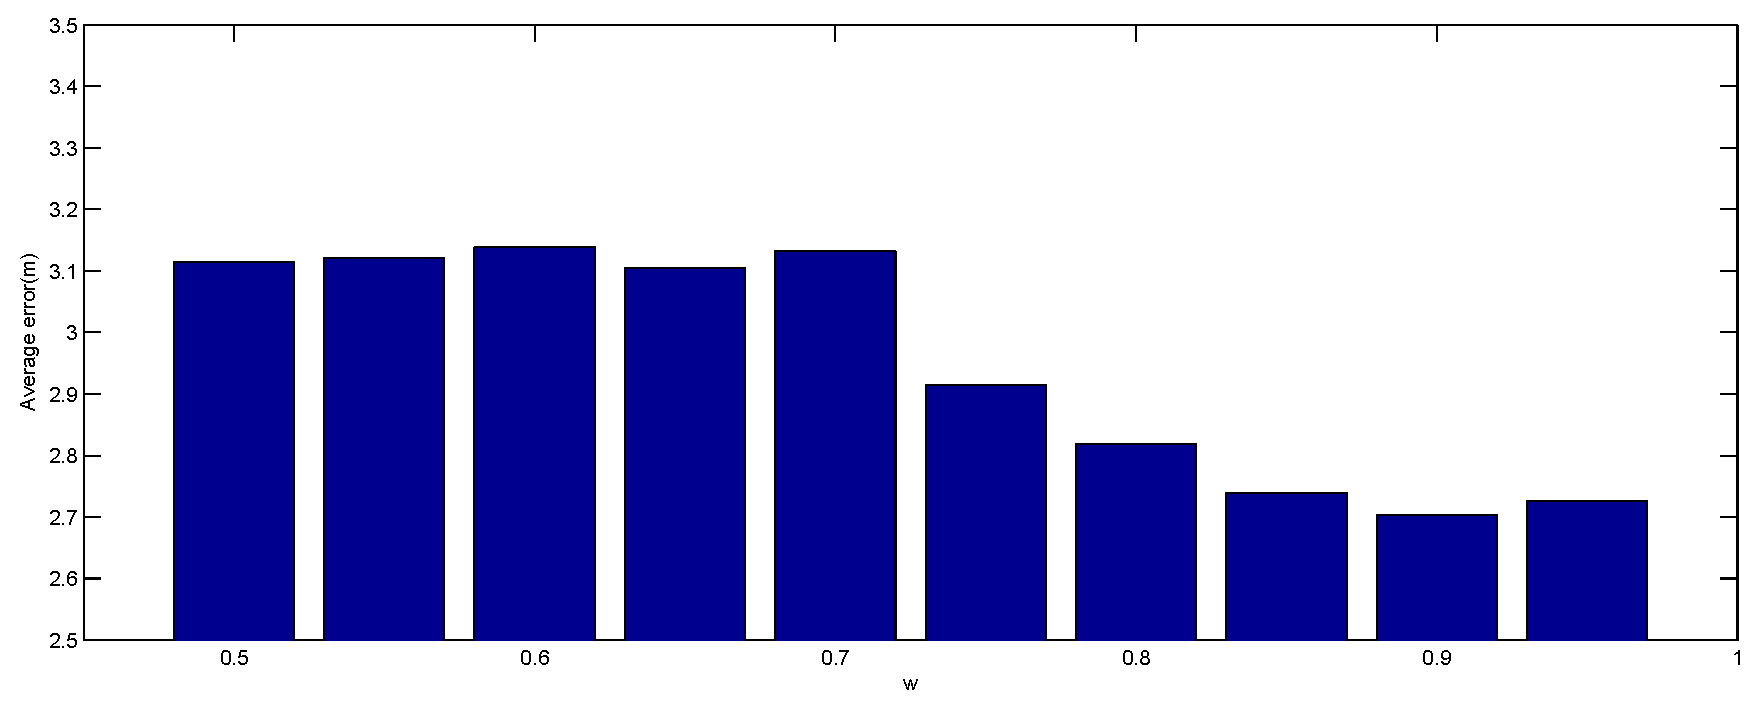
\includegraphics[width=1\linewidth, clip,keepaspectratio]{bar_w_office.eps}
%\caption{Average LE for different $w$.}\label{office_w}
%\end{figure}

%\begin{figure}
%\subfigure[Average error for $w$] {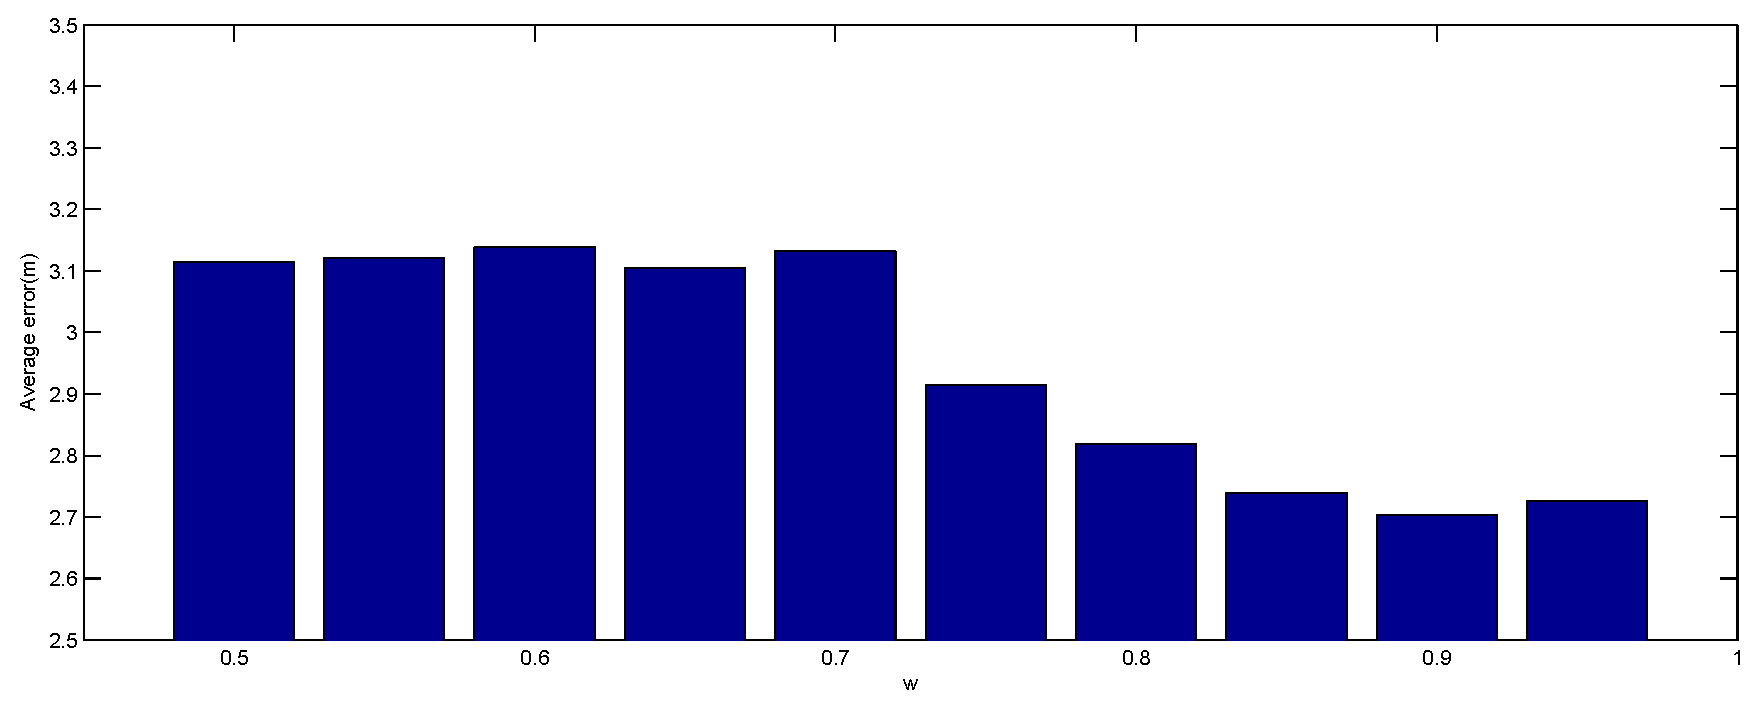
\includegraphics[width=1.4in]{bar_w_office.eps}}
%\subfigure[Avergae error for $t$] {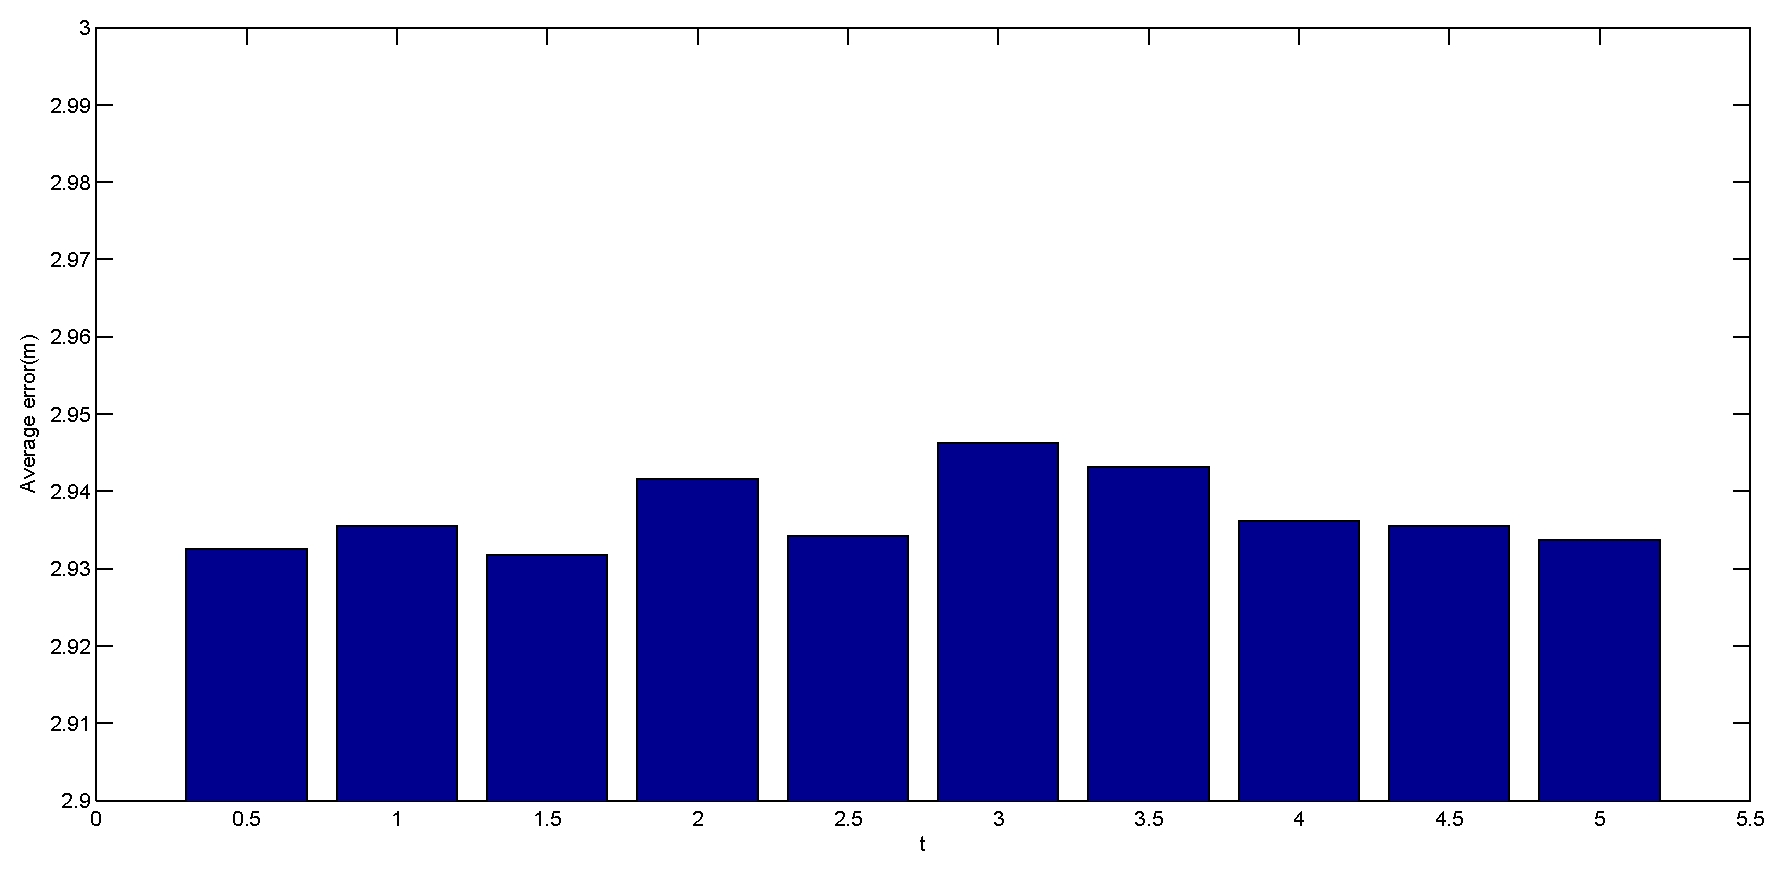
\includegraphics[width=1.4in]{bar_th_office.eps}}
%\caption{Impact of consensus estimate parameters: (a)Average LE for different $w$.(b)Average LE for different $t$.}\label{office_para}
%\end{figure}
\subsection{Case Study \uppercase\expandafter{\romannumeral2}: Shopping Mall}
\subsubsection{Site Survey in Shopping Mall}
We do a site survey for the shopping mall without floor plan, it means that we have to manually mark relative coordinates. Figure~\ref{mall_ref} shows the shooting points by purple diamonds, origin point by red star and filtered reference points by blue crosses. The distance between every adjacent two shooting points is $1.2m$. The shopping mall with $130m\times 13m$ area consists of three little plazas which are connected by two passages. We can tell the shopping mall's structure from the Figure~\ref{mall_ref} which shows the projected reference points.
\begin{figure*}[t!]
\centering
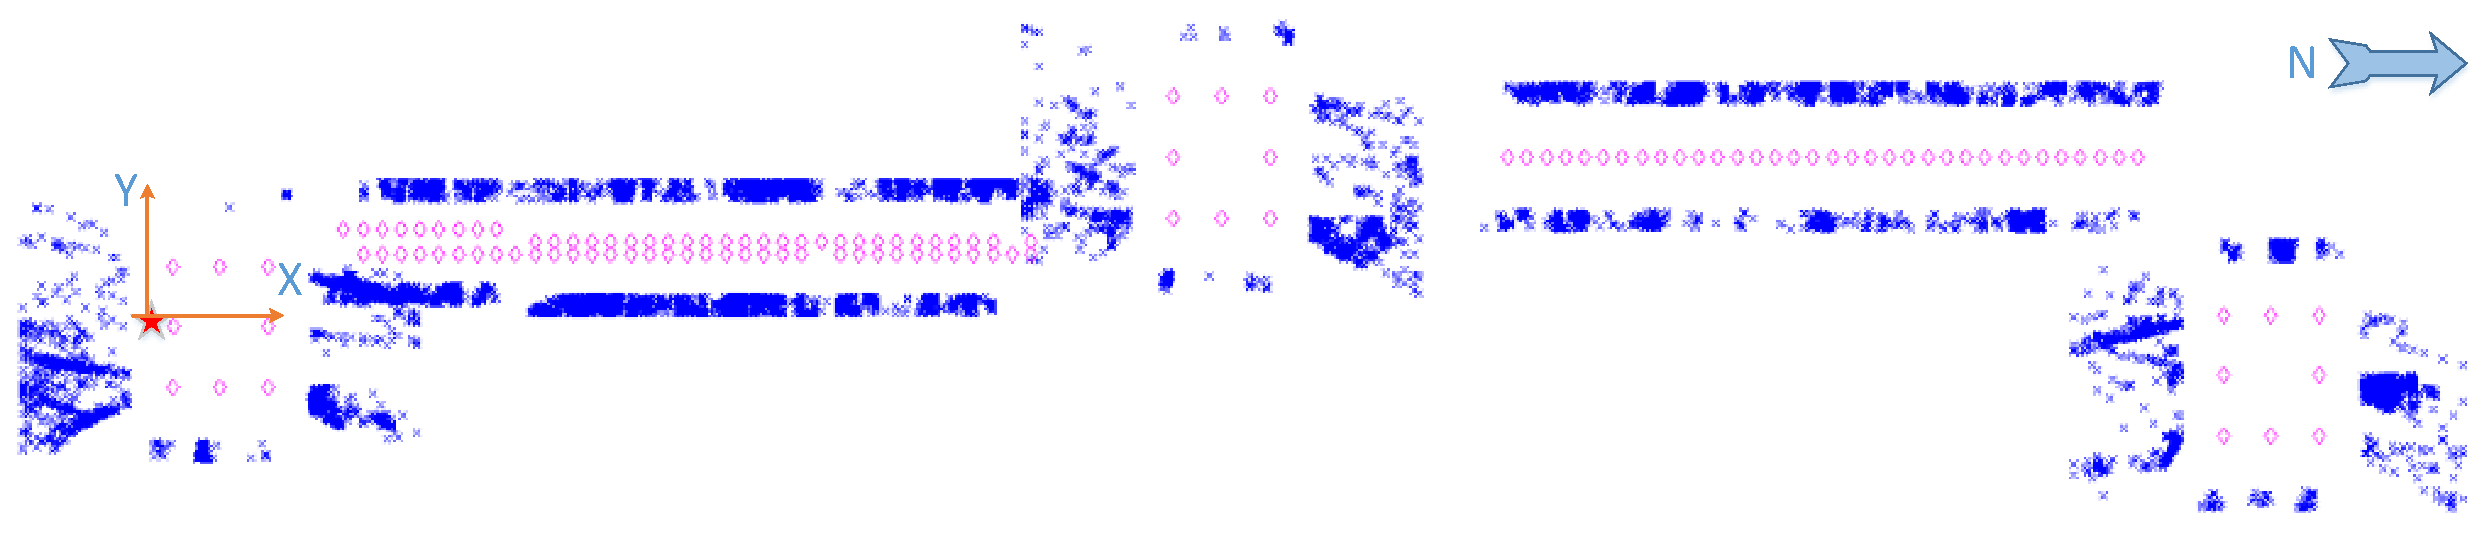
\includegraphics[width=1\linewidth, height=1.1in, clip, keepaspectratio]{mallref2.eps}
\caption{Filtered reference points of shopping mall.}\label{mall_ref}
\end{figure*}
\subsubsection{Reproduction of Results in Previous Work}
In this section, we study the performance of \oursystem in the scenario of shopping mall.
\begin{table}[!htbp]
\centering
\begin{tabular}{ccccc}
\hline
ID &Ref points &Clusters &Time(ms) & \begin{minipage}{2cm}Average cluster size(KB) \end{minipage}\\
\hline
1 &2465 &50 &625 &30.92\\
2 &1739 &42 &516 &26.08\\
3 &1327 &36 &453 &23.36\\
\hline
\end{tabular}
\caption{\label{tab_mall_cluster}Impact of reference point database size on clustering stage for shopping mall.}
\end{table}
Table~\ref{tab_mall_cluster} shows the clustering cost of time and space for a range of size of reference point database in the shopping mall where we conduct experiments on three databases with different sizes.


Figure~\ref{mall_ref_size} shows the localization performance in shopping mall reference point database, which is similar to the results in office environment. As shown in Figure~\ref{mall_ref_size}(a) the AE for database 1 is $2.2m$. The LE run on database1 is $3.4m$ for 90\%, the LT is $1s$ for 90\% as shown in Figure~\ref{mall_ref_size}(b)(c). $Func2$ improves the localization accuracy by $0.7m$ for 90\% queries in shopping mall shown in Figure~\ref{mall_ref_size}(d).
\begin{figure*}
\centering
\subfigure[Average LE]{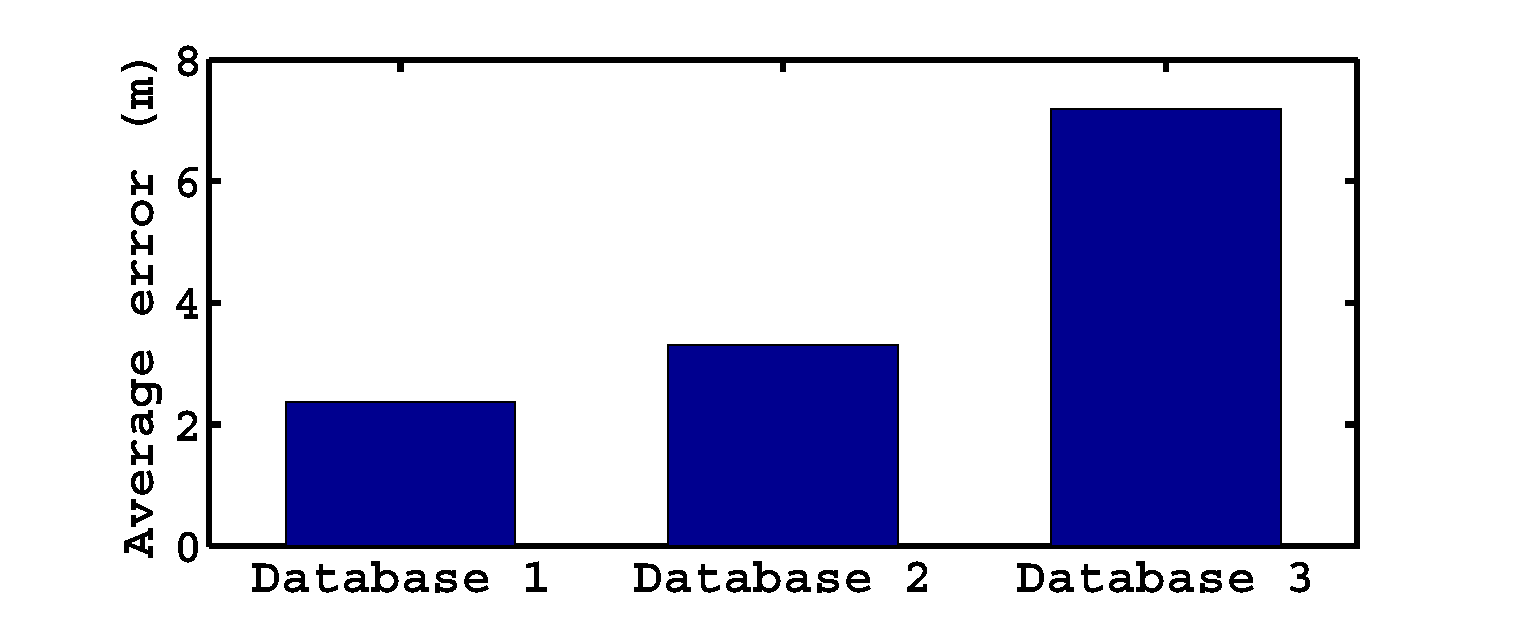
\includegraphics[width=1.7in, height=1.0in]{bar_mall4ds2.eps}}
\subfigure[CDF of LE]{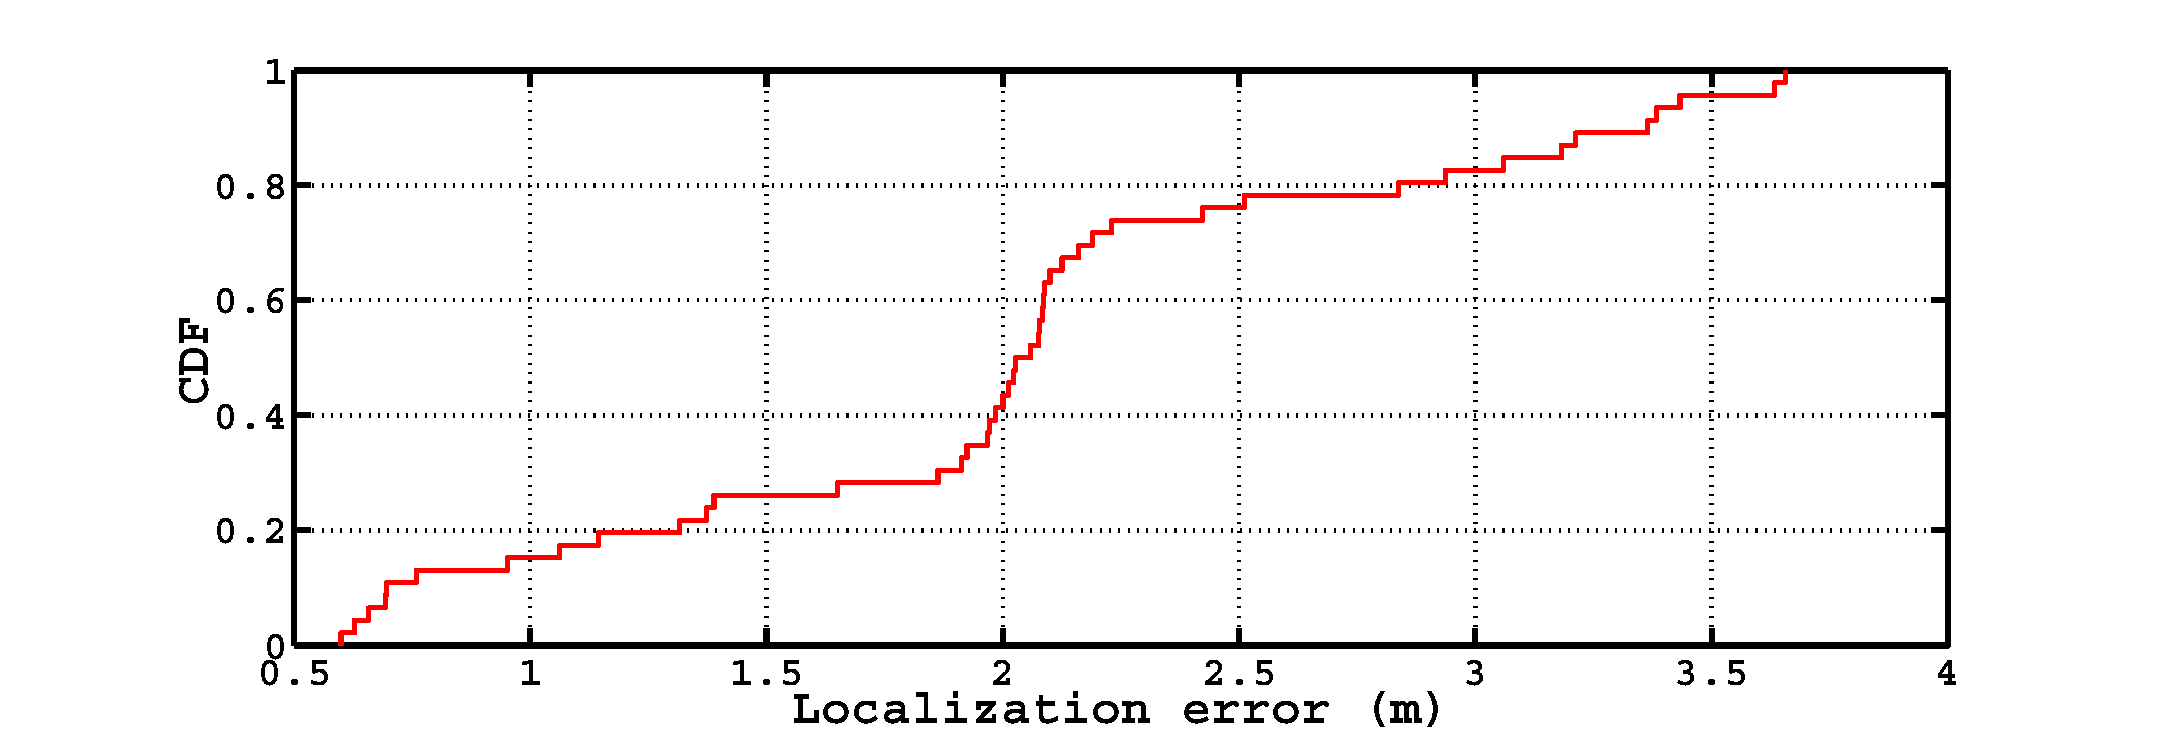
\includegraphics[width=1.7in, height=1.0in]{cdf_mall2.eps}}
\subfigure[CDF of LT]{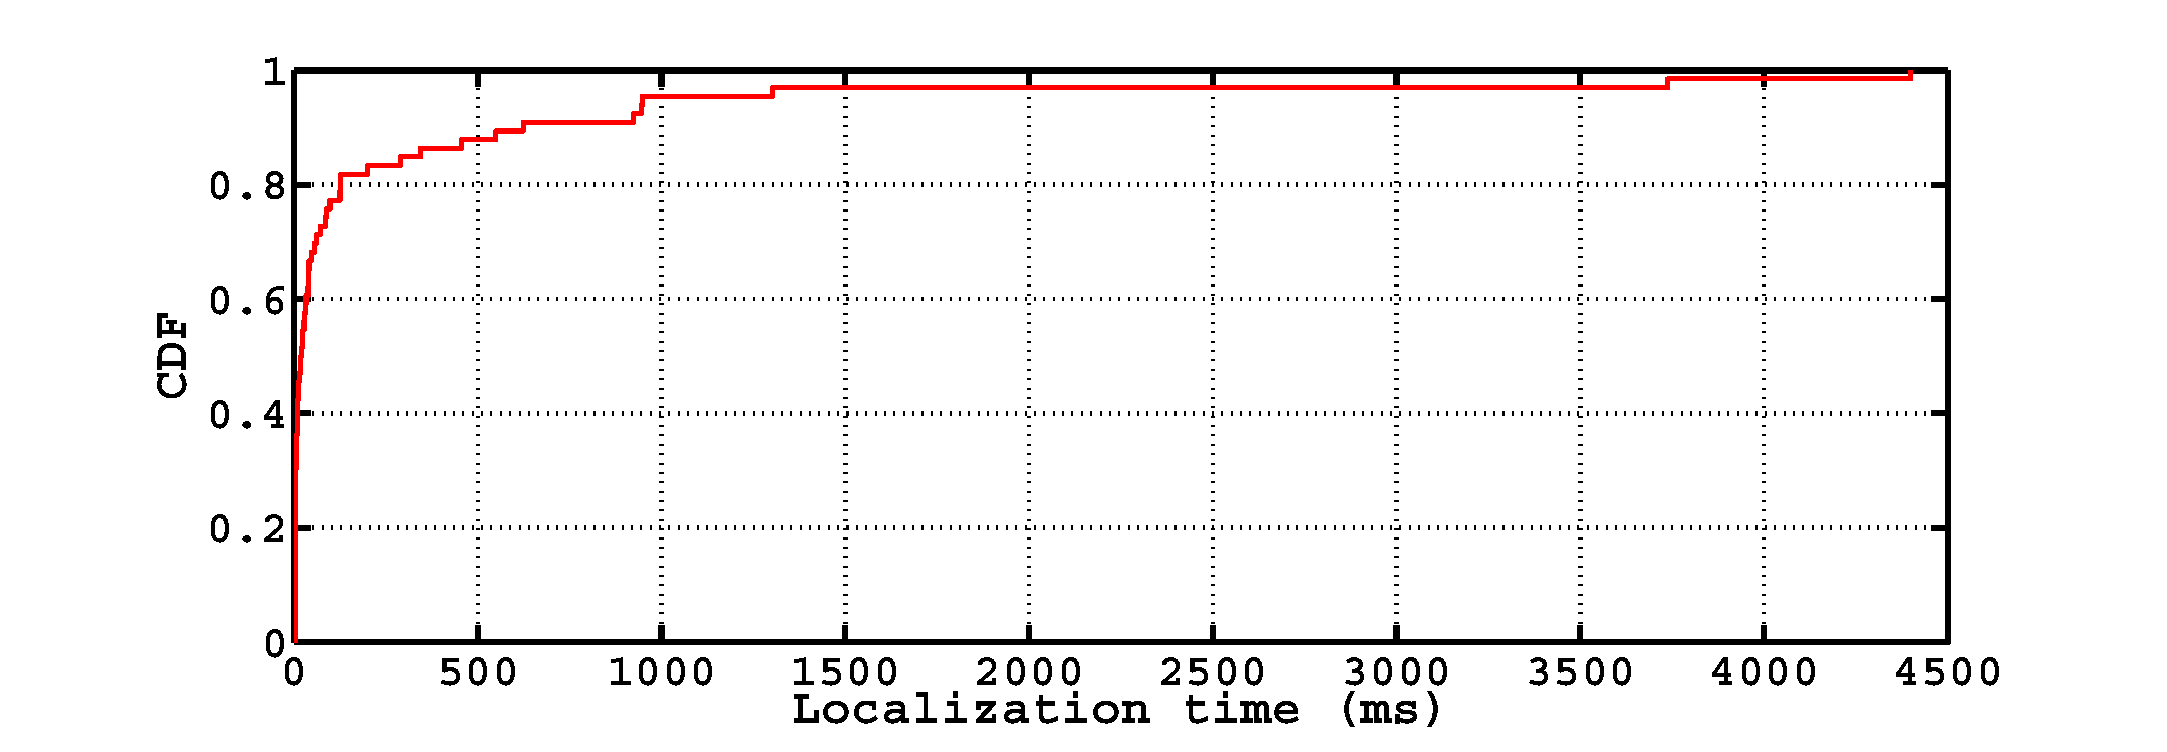
\includegraphics[width=1.7in, height=1.0in]{cdf_malltime2.eps}}
\subfigure[CDF of LE]{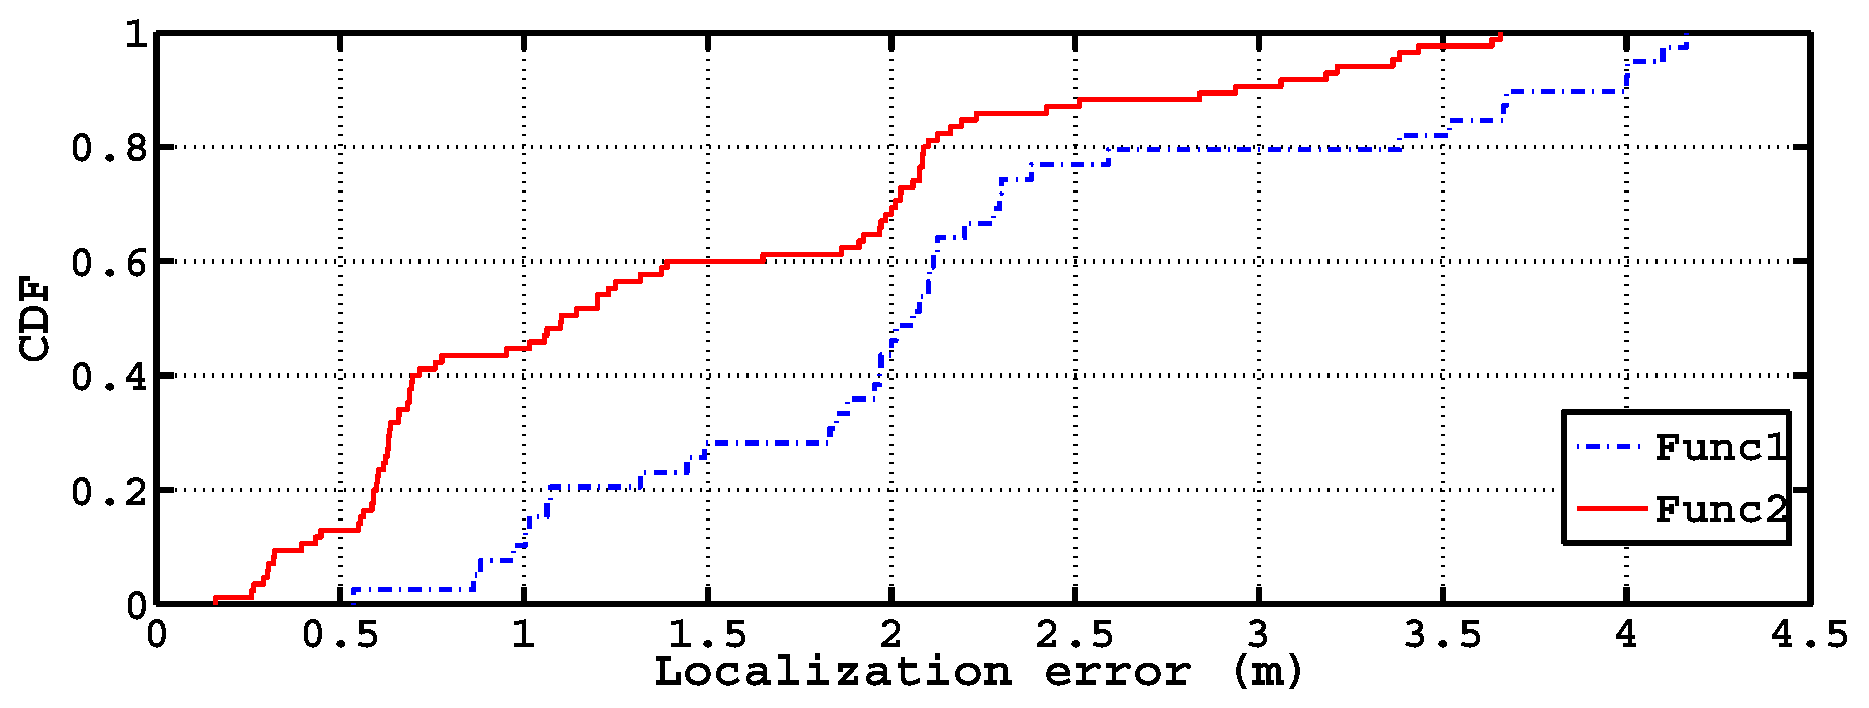
\includegraphics[width=1.7in, height=1.0in]{mall_func12.eps}}
\caption{Localization performance in shopping mall reference points database: (a)Average LE of 3 reference point databases. (b)CDF of LE on database 1. (c)CDF of localization time on database 1.(d)CDF of LE for $Func1$ and $Func2$ in shopping mall.}\label{mall_ref_size}
\end{figure*}
%\begin{figure}[!tbp]
%\centering
%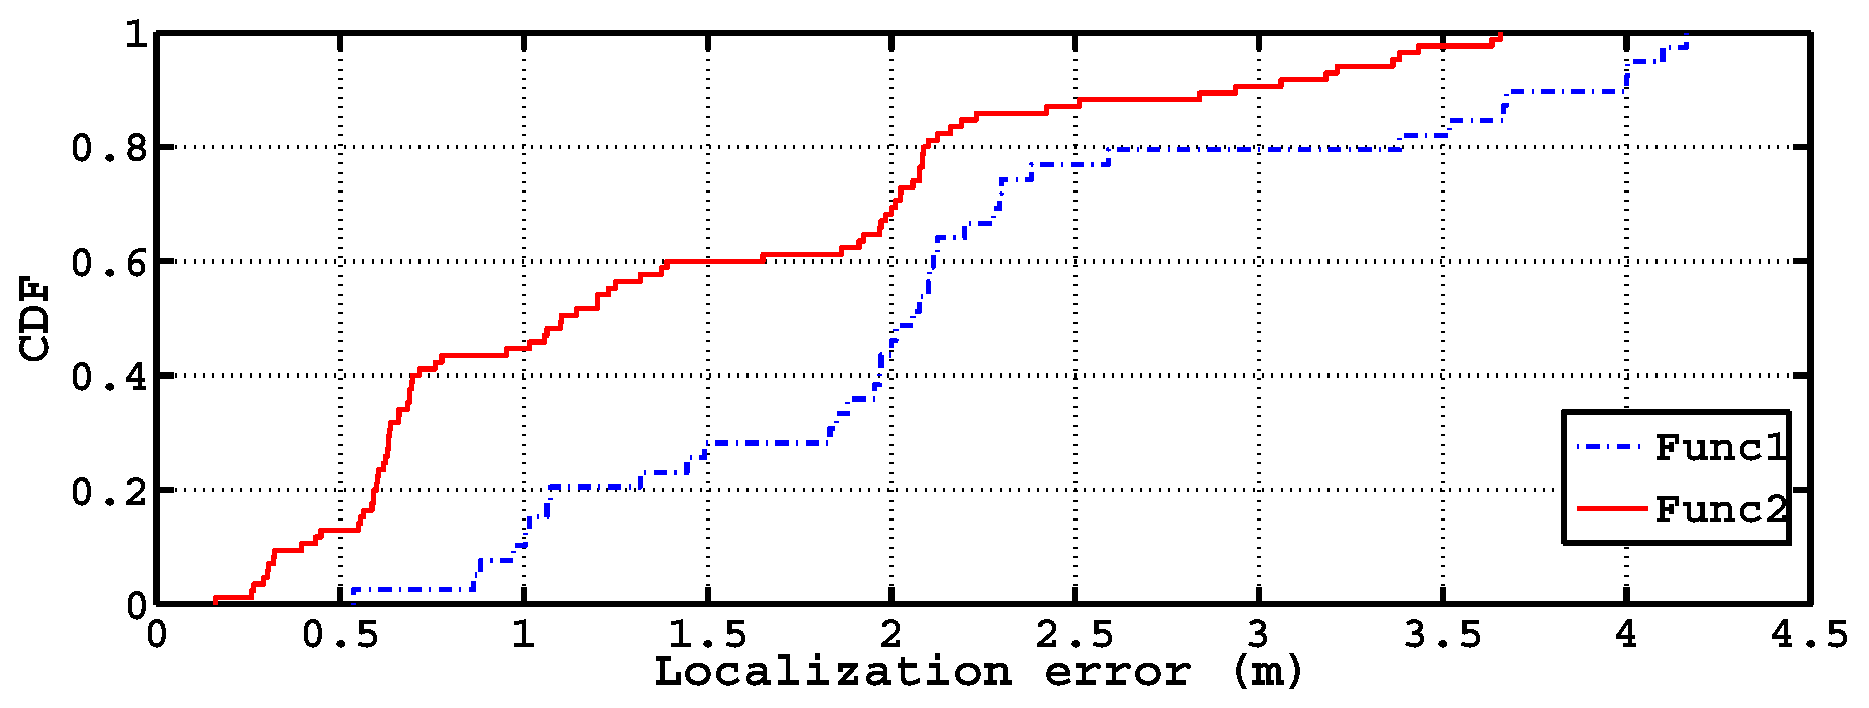
\includegraphics[width=2.2in,height=1.3in, clip,keepaspectratio]{mall_func12.eps}
%\caption{CDF of LE for $Func1$ and $Func2$ in shopping mall.}\label{mall_func12}
%\end{figure}
%\subsection{Communication and Energy Cost}


\section{Related work}
\label{sec:review}
%\textbf{Indoor Localization}
There are many dedicated indoor localization systems with specialized hardware, \eg sensors and RFID,
 which can achieve high accuracy, but are not scalable.
Many application scenarios of mobile social networks are indoor.
One popular line of mobile handset indoor localization is fingerprinting.
These approaches collect fingerprints with known locations
 and compare the observed measurement at unknown locations with
 all known fingerprints to find the best match.
Some systems depend on fingerprints of wireless signals to achieve room-level user localization.
RADAR \cite{bahl2000radar} proposes a radio-frequency (RF) based system
 for locating and tracking users inside buildings.
Horus \cite{youssef2008horus} designs a WLAN location determination system
 which achieves meter-level localization.
\cite{varshavsky2007gsm} presents a GSM indoor
localization system that achieves median accuracy of 4 m.
Some recent systems have incorporated surveying by users.
OIL \cite{park2010growing} uses Voronoi regions for conveying uncertainty and reasoning about gaps in coverage, and a clustering method for identifying potentially erroneous user data to facilitate rapid coverage while maintaining positioning accuracy.
EZ \cite{chintalapudi2010indoor} exploits the RSSI of indoor APs to estimate the user's location with no pre-deployment effort and yield a median localization error of 2m and 7m.

%There are other types of fingerprints used to achieve room-level localization.
%For example, SurroundSense \cite{azizyan2009surroundsense} proposes
% a system for logical localization (like Starbucks, McDonalds)
% using optical, acoustic, and motion attributes sensed by
% the phone as a logical location fingerprint.
%\cite{matic2010tuning} uses FM radio signal as the fingerprint,
%Batphone \cite{tarzia2011indoor} uses a ambient sound fingerprint
% called the Acoustic Backgroun Spectrum (ABS),
% \cite{chung2011indoor} uses Geo-magnetism as fingerprint,
% \cite{jin2010indoor} uses CIR(channel impulse response) as fingerprint.

Some work localize by estimating distances to anchor nodes
 based on RSSI, time-of-arrival (TOA), time-difference-of-arrival (TDOA) and angle-of-arrival AoA.
BeepBeep \cite{peng2007beepbeep} proposes ETOA which enable a centimeter accuracy acoustic-based
 ranging method between a pair of mobile handsets.
ETOA avoids many sources of inaccuracy found in other typical time-of-arrival
schemes, such as clock synchronization, non-real-time handling,
software delays, etc.

\cite{qiu2011feasibility} presents a solution for achieving high speed 3D continuous
localization for a pair of phones using two microphones with one
speaker on a phone. This approach uses acoustic cues based on time-of-arrival and
power level with assistance of accelerometers and digital compasses.
\cite{liu2012push} obtains acoustic ranging estimates
among peer phones and maps phones' locations jointly against
 WiFi signature map subject to ranging constraints
 to reduce the significant errors of WiFi-based method.
Virtual Compass \cite{banerjee2010virtual} designs a
 peer-based relative positioning system on commodity mobile handhelds
 to determine proximity.
It uses multiple radios to detect nearby
 mobile devices and places them in a two-dimensional plane.
It uses adaptive scanning and out-of-band coordination to explore trade-offs between
energy consumption and the latency in detecting movement.

%\cite{pierre2001deriving} extracts the edges and color features and encodes them as fingerprint sequence.
% then makes use of a sequence matching algorithm to find the best match between the query image and the pre-built panoramic view database of the scene to determines the location where the query image was taken.
% The system needs a exhausted site survey to pre-build a panoramic view database which makes use of specific devices.
%Mobile phone,sensor hints: accelerometer, compass, gyro, camera, microphone noisy, logical localization,body blocking effect.
%feature: power:RSSI:wifi, time:TDoA:uwb, angle:AoA:mimo
%mobile phone,sensor hints: accelerometer, compass, gyro, camera, microphone
%noisy, logical localization
%RSSI:path loss ,shadow, multipath
%RSSI dynamic, rssi changes during a short period
%body blocking effect
%\textbf{User Pattern Preconization}
%\textbf{Neighbor Discovering}
%Centralized: Provides applications with absolute locations.
%Indoor localization is difficult.
%It is slow and difficult to manage across applications.
%Mobile to mobile: QualComm AllJoyn, Nokia Sensor, Nintendo StreetPass, Sony Vita, Wi-Fi Direct
%Local, reduced latency, up-to-date, user-controlled.
%It enables applications to focus on proximity instead of absolute location.
%challenge:encounters are unplanned and changing, constant scanning is energy consuming.
%Efficient duty cycling requires global synchronization which is difficult.
%(Small delay required)
%
%\textbf{Classification based Localization}
%\cite{iwan2000appear} recognizes mobile robot's topological position by voting from the color bands combined to classify the input images. The system classifies the input images in real-time based on nearest-neighbor learning, image histogram matching and a simple voting scheme.
%\cite{kosecka2003qual} presents a qualitative localization scheme. The system firstly infers a topological model of an environment from images or video streams, then classifies the image according to gradient orientation histograms of image's edge map. At last, the system determines the location taking advantage of Learning Vector Quantization(LVQ) which obtained by selecting the representative feature vectors best covering the class.

%\textbf{3D model based Localization}
%Construction: expensive; Matching: expensive; Storage: large data size.
%Existing work: pinhole model based ranging.
Structure from Motion(SfM) reconstruction approaches enables the creation of large scale 3D models of urban scenes\cite{torsten2011fast}, which can be used in image-based localization through computing 2D-to-3D correspondences.
To improve the performance of 2D-to-3D matching methods, \cite{torsten2011fast} derives a visual vocabulary quantization based matching framework and a prioritized correspondence search. Compared with SfM, \oursystem builds up the reference points database by binocular ranging which combines the position of shooting point with feature point 3D coordinates computation. In this way, \oursystem reduces the error of 3D structures of indoor environment.

\cite{jason2013image} presents a pipeline system to perform image-based localization of mobile devices.
A 3D geo-referenced image database is generated by making use of a specific human operated backpack.
It matches SIFT feature extracted from query images against the 3D point cloud, combining user's cell phone sensor information like pitch and roll, to recover the user's pose.

Some vison-based localization works\cite{kosecka2003qualitative}\cite{kosecka2003qualitative}\cite{ulrich2000appearance}compares a test image against a database of pre-captured benchmark images, finds the "closest" match and uses its location. \cite{tian2014towards} combines photos and gyroscope on smartphone to localize users by measuring users' relative positions to physical objects. \cite{manweiler2012satellites} allows users to locate remote objects by a few photos from different known locations.


\section{Acknowledgements}
\label{sec:ack}
This research is supported by NSF China Major Program under Grant No.61190110. 
We thank all the reviewers for their valuable comments and helpful suggestions.

\section{Conclusion}
\label{sec:conclusion}
In this work, we study the problem of building a practical system which provides realtime and accurate indoor localization service for smart phone users. While many innovative proposals have been presented in the literature, we take advantage of the SURF vision feature and perspective projection model to build reference point database and to perform indoor localization without deploying any infrastructure. Our approach is simple but works effectively to provide localization service in indoor environment with reasonable accuracy. We further improve the accuracy using enhanced estimate check function $Func2$. Through all processes of \oursystem, there is not much expenditure in time and cost for site-survey or running the system. We are convinced that our proposal can suggest a new approach combining computer vision technique with indoor localization research.


%\fontsize{21pt}{\baselineskip}\selectfont
%\begin{spacing}{0.85}
% references section
{\small
\bibliographystyle{IEEEtran}
\bibliography{sigproc}
}
%\end{spacing}





\end{document}
